\chapter{Verifying Direct Volume Rendering Algorithm}
\label{chap:vr}

Over the past decades, the visualization and graphics communities have developed a wide range of volume rendering techniques. As they are used in different disciplines of science, and thus form a basis for new scientific insights, it is essential to assess their reliability and identify errors. Furthermore, the increasing complexity of volume rendering algorithms makes the correctness of the algorithm itself as well as its potentially error-prone implementations complementary and equally important issues. Especially in areas such as medical imaging where accuracy and precision play a crucial role, a formal methodology for assessing correctness is highly desirable~\cite{kirby-vv-08, Pommert2002}. While verification is widely adopted in different branches of computer science -- see  model checking~\cite{Clarke08}, fuzzing~\cite{godefroid08}, and convergence analysis~\cite{Roy2005} -- not much work on a formalized praxis for asserting the correctness of visualization techniques has been done. 
%Among the existing techniques, there are three conceptual approaches which could be applied to assess the reliability of volume rendering techniques, i.\,e., algorithm comparison~\cite{Meissner:2000:PEP:353888.353903}, error estimation~\cite{Moller:1996:CLE:236226.236235} and uncertainty visualization~\cite{Johnson:2003:NSV:942583.942610}. 
In this chapter we present a new verification approach for direct volume rendering techniques as well as its theoretical background. 
%We use the word verification in the same sense Babuska and Oden \cite{babuska04}: ``verification is the process of determining if a computational model, and its corresponding numerical solution, obtained by discretizing the mathematical model (with corresponding exact solution) of a physical event, and the code implementing the computational model can be used to represent the mathematical model of the event with sufficient accuracy''~\cite{babuska04}. 
The presented methodology is based on order-of-accuracy and convergence analysis~\cite{Roy2005} which we can apply after deriving the expected behavior of the algorithms under observation. 

To allow the verification of volume rendering algorithms, we start with an analysis of the volume rendering integral and the most common discretization of this continuous model. This analysis gives us insight into expected behavior of the observed algorithms, which is essential to perform a verification~\cite{159342}. In this sense, our main assumption, serving as a foundation for the proposed verification approach is that discretization errors of the implementations under verification should behave as the errors introduced by 
the discretization of the volume rendering integral. 
Based on this, we can mathematically derive the expected behavior from the discretization of the volume rendering integral and verify existing implementations through convergence analysis, by comparing their actual behavior to the expected behavior. 
%In practice, this verification process is performed by applying parameter sweeping, extracting the convergence curves and comparing them to our predictions. 
Based on the results of this comparison, we can assess the correctness of the implementation under verification. To get further insights about deviation from the expected behavior, we present an investigation of the sensitivity of this method. 
%To do so, we discuss error classes and address if these can be successfully detected by the proposed verification methodology. 
Thus, we can demonstrate that our methodology is capable of increasing the confidence in volume rendering algorithms. To our knowledge, the proposed approach is the first step towards the verification of DVR algorithms. Thus, it can be seen as an important contribution towards a formal verification methodology of volume rendering techniques~\cite{roach98}.
% which has the ultimate goal of deriving a correctness guarantee~\cite{Roache_1998}. 
The main contributions of this chapter are:
\begin{itemize}
\item we derive the theoretical foundations necessary for verifying volume rendering with order-of-accuracy and convergence analysis. We analyze the volume rendering integral and its discretization to derive an algorithm's expected behavior when being subject to parameter changes.
\item we explain how to exploit this theoretical foundation to perform a practical verification of implemented volume rendering algorithms, such that it can be easily used for the verification of existing volume rendering frameworks;
\item we discuss the limitations of the proposed concepts by analyzing frequently occurring errors and by documenting those errors we could identify when applying the presented methodology to two widely used volume rendering frameworks, 
\text{VTK} \cite{vtk} and Voreen \cite{MRMH09} (see Figure~\ref{chap5:fig:teaser}).
\end{itemize}

\begin{figure}[b]
\centering
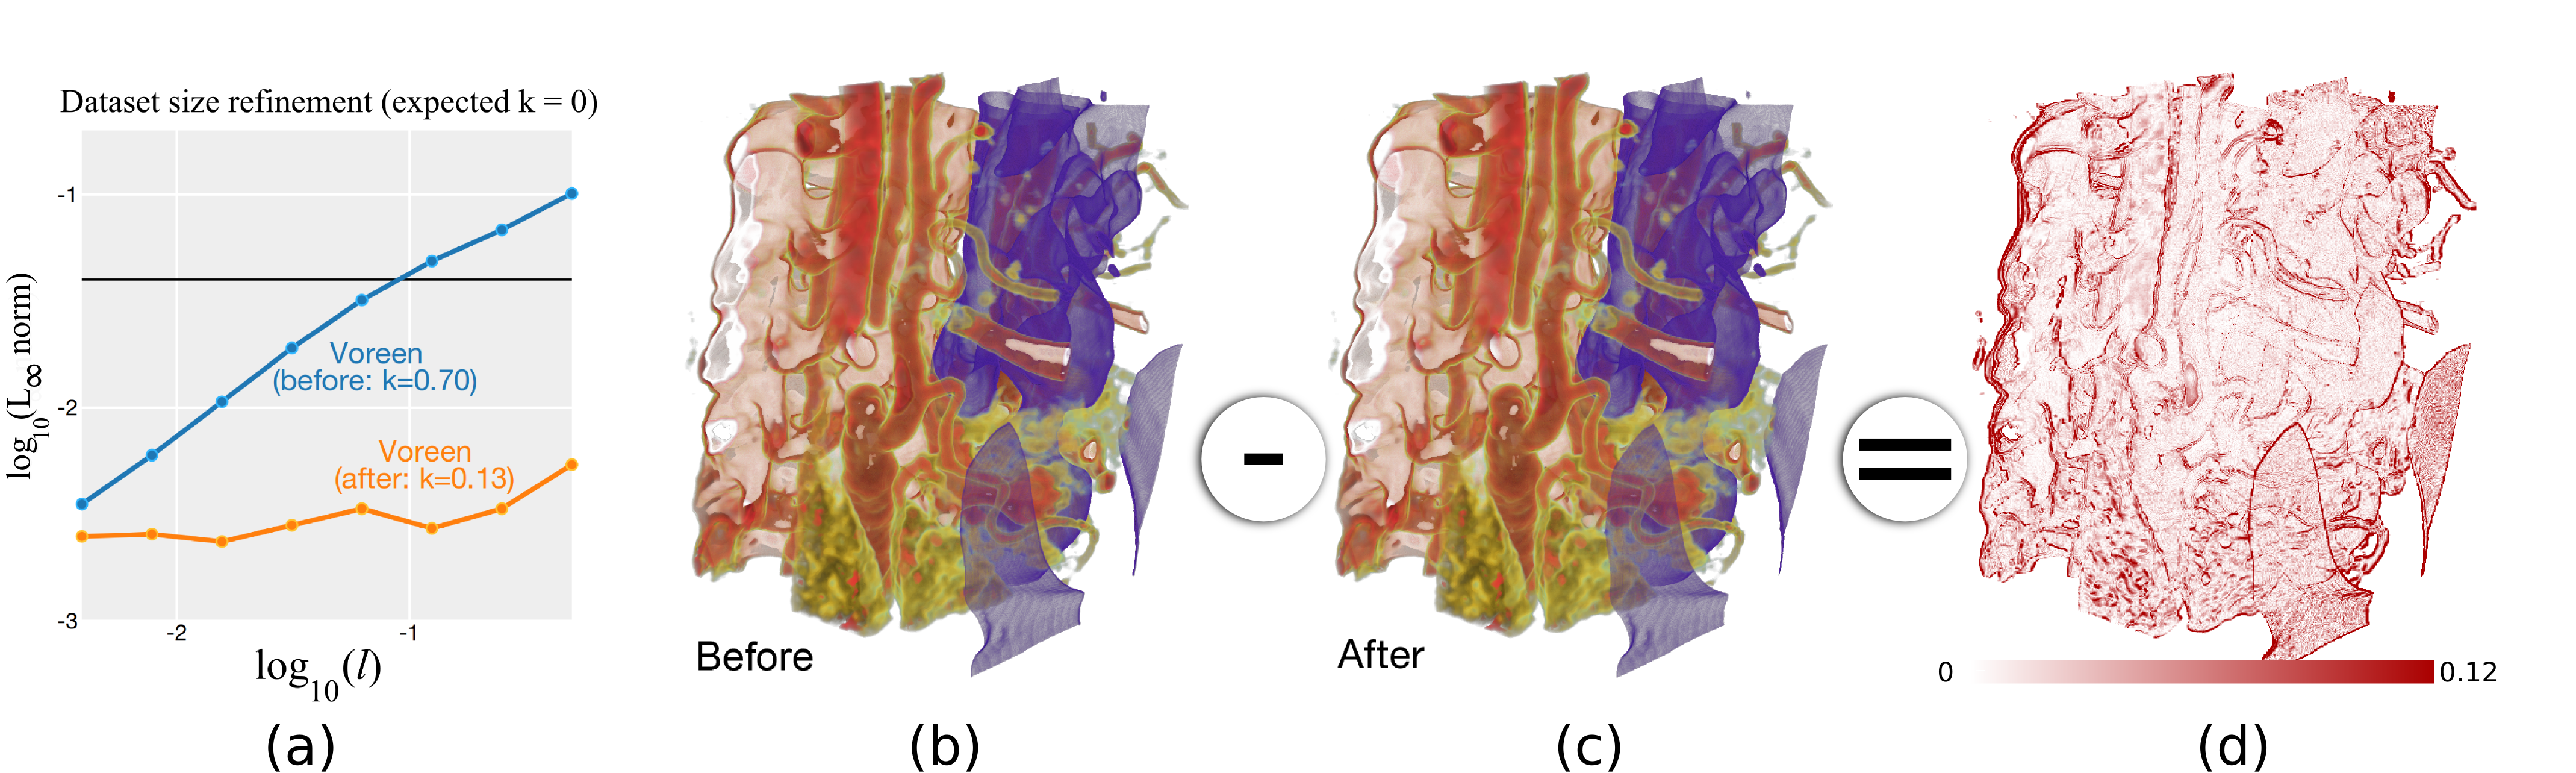
\includegraphics[width=1\linewidth]{chapter5/figures/teaser.png}
\caption{\label{chap5:fig:teaser} (a) shows the result of our verification procedure
  for dataset refinement. The
  blue line corresponds to the initial behavior, which deviates from
  the expected slope (solid dark line).  After fixing
  the issues, we obtain the orange curve, with a slope closer to the
  expected one (denoted by $k$). (b) and (c) show a
  human torso, displaying the blood vessels and the spine, before and
  after our changes.  (d) shows the difference between (b) and (c).}
\end{figure}

%%The following has been removed for the sake of space
%%The paper is structured as follows. After discussing related work and
%%challenges in Sections~\ref{sec:related-works} and
%%\ref{sec:verification}, we present the theoretical concepts needed to
%%verify volume rendering algorithms based on the discretization error
%%analysis in Section~\ref{sec:volume-rendering}. The actual convergence
%%analysis is then presented in
%%Section~\ref{sec:convergence_analysis}. Section~\ref{chap5:sec:results}
%%discusses our results, which we have achieved by applying our approach
%%to existing volume rendering frameworks, namely VTK and
%%Voreen. This analyses allowed us to identify unexpected
%%behavior and solve the underlying problems, as it is depicted in
%%Figure~\ref{chap5:fig:teaser}. In Section~\ref{chap5:sec:discussion} we provide a
%%detailed discussion of our findings and their implications, before we
%%address the limitations of our approach and conclusion in
%%Sections~\ref{sec:limitations} and \ref{sec:conclusion}.

%According to IEEE standards, \emph{verification} is the ``process of evaluating a system or component to determine whether the products of a given development phase satisfy the conditions imposed at the start of that phase''~\cite{159342}.

%One may be tempted to classify the verification as debugging, a well-known process for finding software glitches. Although debugging has been used extensively in computer science (and hence in the visualization community), our claim is not that the debugging process has not been used in visualization but that there are only a few attempts to formally verify correctness of visualization implementation.

%Clearly, our approach is problem-dependent, but its general formulation can be applied not only to isosurfacing and volume rendering, but also to techniques such as streamline computation and mesh simplification. In this chapter, however, we focus on direct volume rendering.

%We emphasize that verification is a \emph{process}. Our goal is to increase confidence in a given implementation rather than prove or provide any final guarantees on the implementation correctness~\cite{Roache_1998}. The latter is known in computer science as formal verification~\cite{FLO67,Hoare:1969:ABC:363235.363259} an approach beyond the scope of this work.


\section{Related work}
\label{sec:related-works}

Critical decisions in fields such as medical imaging often rely on
images produced by volume rendering algorithms, where it is of utmost
importance that the results are correct~\cite{Duncan2000}.  The
multitude of algorithms components and their interactions make
this guarantee a challenge. As a consequence, many authors focus on specific
aspects of the problem such as numerical aspects of the evaluation of
the volume rendering integral, shading, transfer functions, and
interpolation schemes.  The quality of volume rendering has always
been of central interest to the community, and relying on visual
inspection is a common practice. Meissner \emph{et
al.}~\cite{Meissner:2000:PEP:353888.353903} evaluate volume rendering
techniques using the human visual system as a reference while, more
recently, Smelyanskiy \emph{et
al.}~\cite{Smelyanskiy:2009:MHV:1638611.1639155} present a domain expert guided comparison scheme.
%that uses an evaluation guided by a domain expert.  
While those approaches are valuable, the need for a more systematic
evaluation is discussed in several
papers~\cite{globus95,Johnson:2004:TSV:1018014.1018051,Johnson:2003:NSV:942583.942610,kirby-vv-08}. See Pommert and
H\"{o}hne~\cite{Pommert2002,Pommert2003} for a survey.

Among several aspects to consider in the correctness of volume
rendering algorithms, one of the most important is the approximation
of the volume rendering integral. The solution with linearly
interpolated attributes is presented by Williams and
Max~\cite{Williams1992}, with further discussions on its numerical
stability by Williams \emph{et al.}~\cite{Williams1998}.  Interpolant
approximations and
errors~\cite{Hajjar08,Moller:1996:CLE:236226.236235,Moller1997,Novins:1992:CPV:147130.147154},
gradient computation~\cite{Alim2010} and opacity
correction~\cite{Lee2007} are also the subject of analysis with regard
to numerical accuracy. The idea of \emph{pre-integration} enabled
high-quality, accurate and efficient algorithms using graphics
hardware~\cite{Engel01,Kye:2008p871,Rottger2000}. Similarly, VTK
currently uses partial pre-integration, in particular for unstructured
grids~\cite{Moreland2004}. Note that although there has been work on
high-order and high accuracy volume rendering, to the best of our
knowledge none of these approaches attempted to evaluate the convergence
rate of the standard discretization process of the volume rendering integral, thus providing
weaker mechanism to evaluate whether or not the mathematical foundations of the algorithms
have been implemented in a correct manner.

The use of a verification framework has only recently been discussed
in scientific visualization, despite the vast literature on
verification in computer science. Globus and Uselton~\cite{globus95}
first pointed out the need to verify not only visualization algorithms
but also their implementations, and Kirby and Silva suggested a
research program around verification~\cite{kirby-vv-08}. The
verification of isosurface algorithms is discussed by Etiene \emph{et
al.}~\cite{Etiene:2012:TVI:2197070.2197097, etiene:tvcg:2009}, where a systematic evaluation identified and
corrected problems in several implementations of isosurface extraction
techniques.  Zheng \emph{et al.}~\cite{Zheng10} address CT reconstruction and
interpolation errors in direct volume rendering algorithms using a
verifiable framework based on projection errors. In contrast, our work
focuses on the verification of the final image produced through direct
volume rendering.

\begin{figure}[b]
\centering
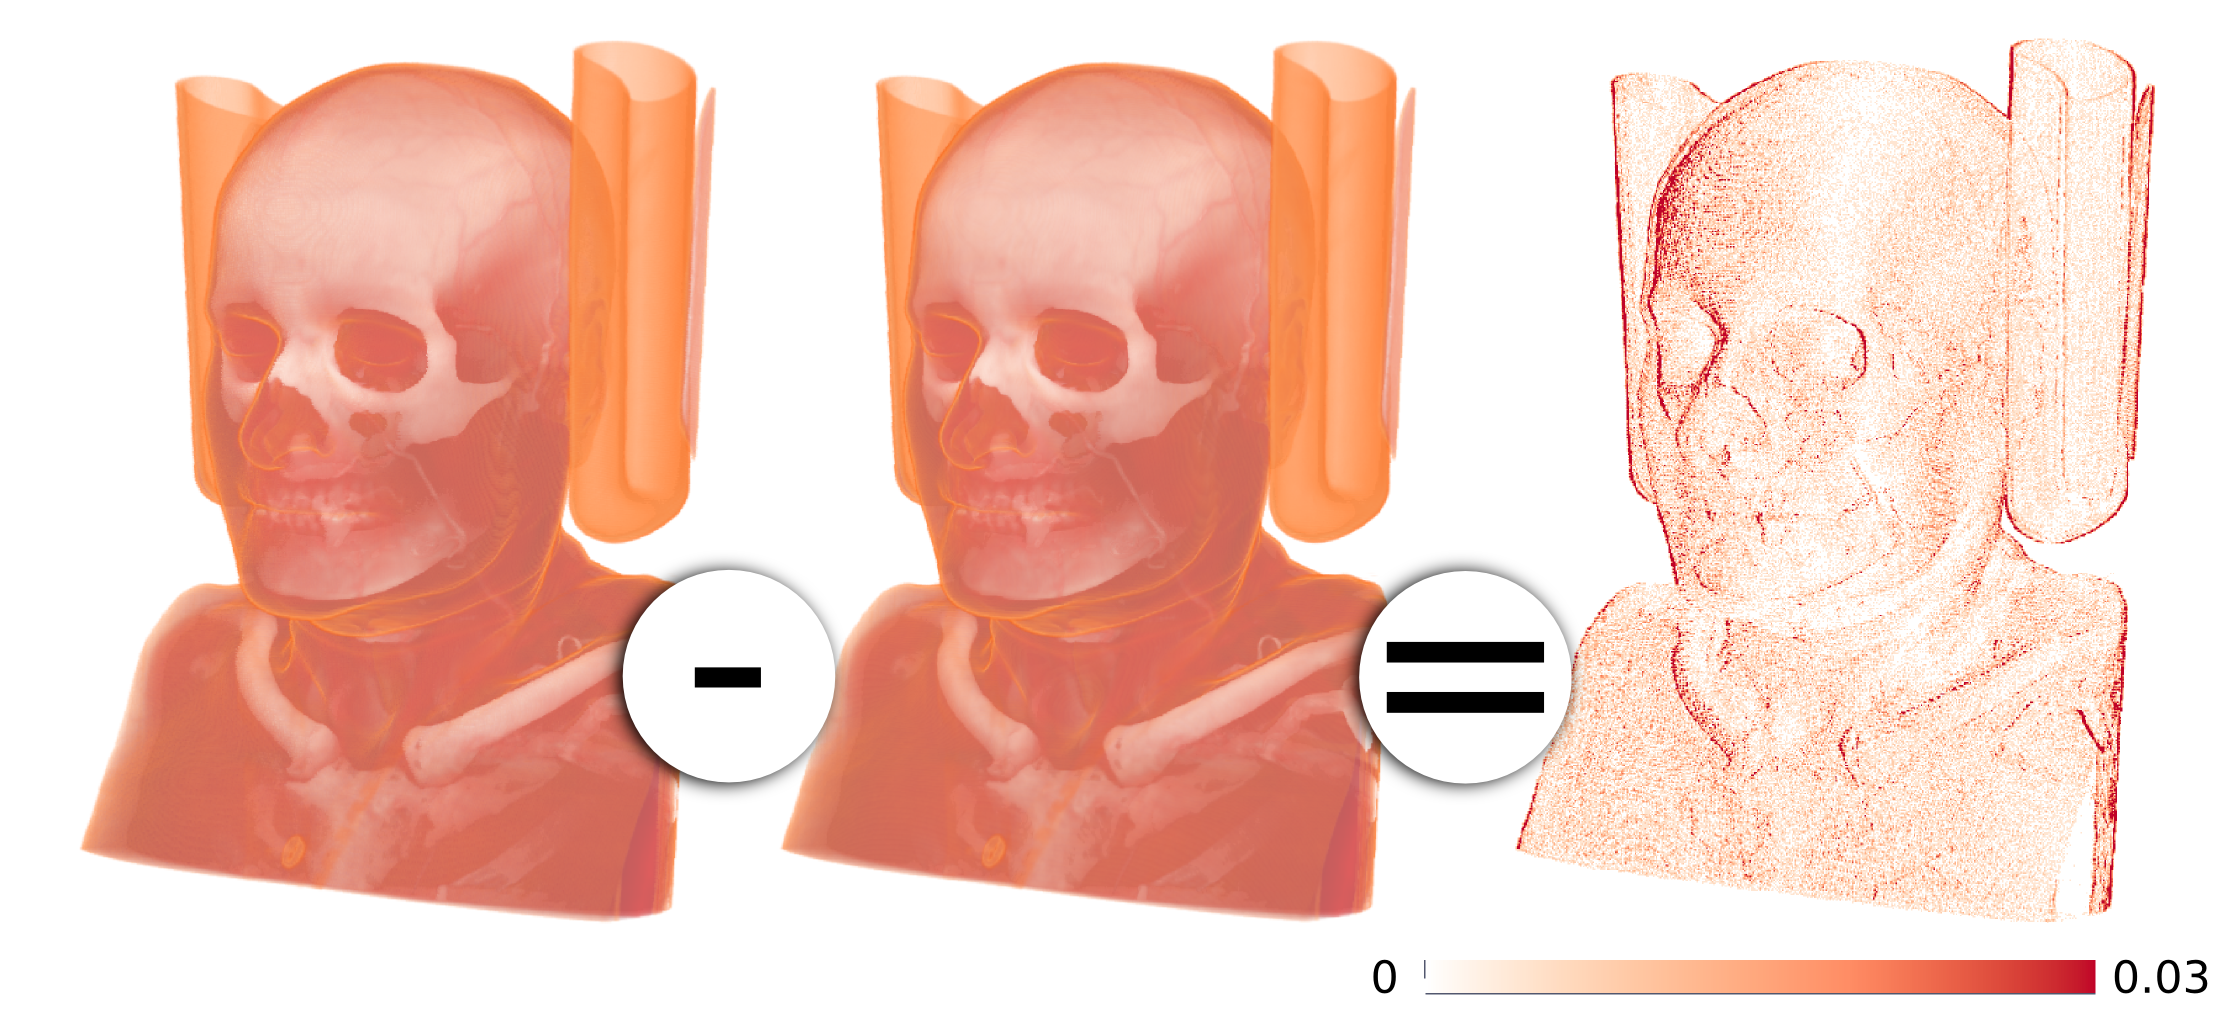
\includegraphics[width=1\linewidth]{chapter5/figures/torso-image.png}
\caption{\label{fig:error-quantification-examples}  Left: 
  the volume rendering of the torso dataset with incorrect trilinear
  interpolant. Middle: Same dataset with the correct 
  interpolant. Right:  image shows
  the difference between them.}
\end{figure}

\section{Verification}
\label{sec:verification}

Before presenting our verification procedure, let us consider four of
the techniques used for code verification in computational
science~\cite{Roy2005}: \emph{expert judgment}, a procedure in which a
field expert determines if the output of an implementation is correct
by evaluating the results; \emph{error quantification}, which is the
quantification of the discretization errors when compared to an
analytical solution, a benchmark solution or some ground-truth;
\emph{convergence analysis}, a procedure in which one evaluates if the
discretization errors converge to zero as a function of some
parameter; and \emph{order-of-accuracy}, a procedure where one
evaluates if the discretization errors decrease according to the
expected rate. In this list, the expert judgment is the least rigorous
test, followed by error quantification and convergence analysis. 
Order-of-accuracy is widely recognized as the most rigorous code
verification tool~\cite{babuska04, KnuppSalari02, roach98,
  Roy2005}. In this chapter, we focus on the last two methods, namely,
convergence analysis and order-of-accuracy. Before we dive into these
methods, let us first consider some of the limitation of the expert
analysis and error quantification.
\begin{figure}[b]
\centering
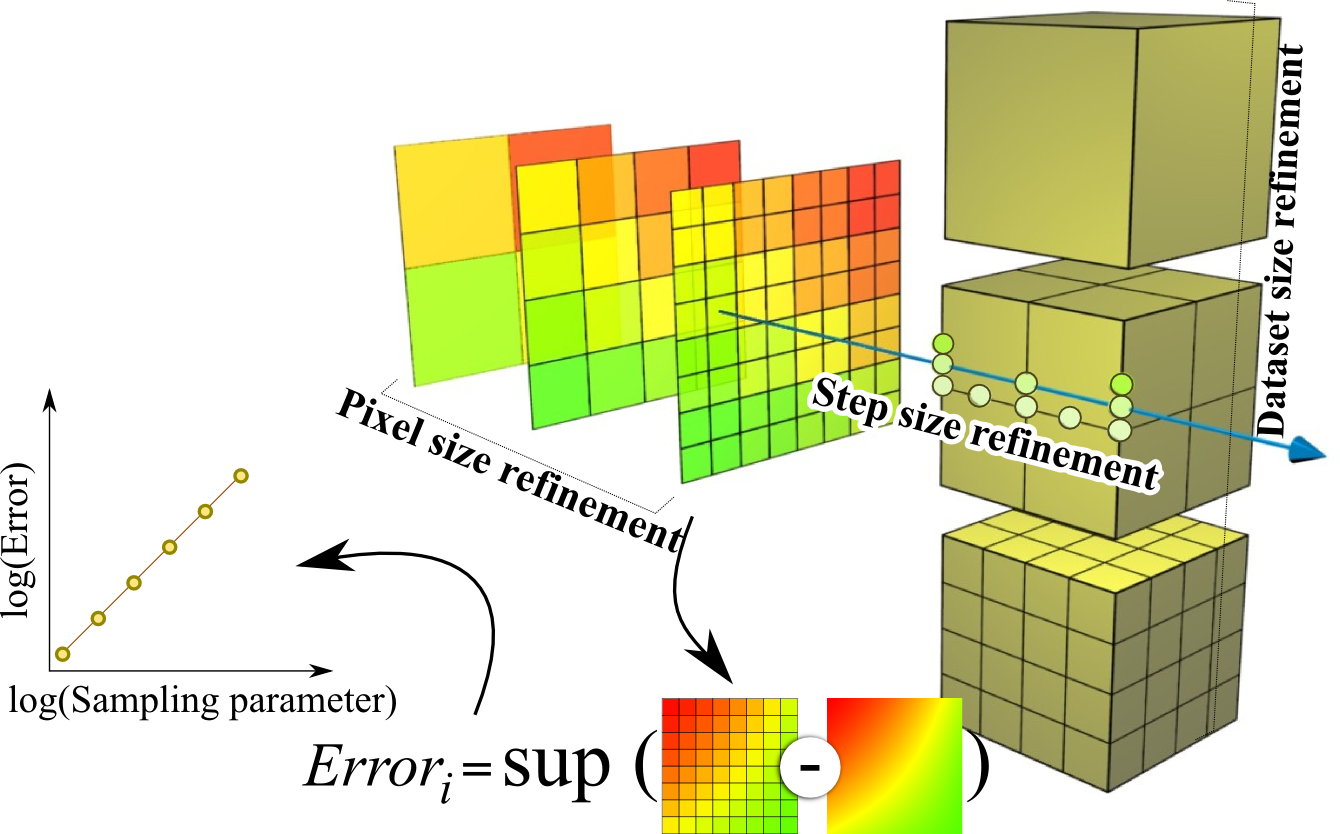
\includegraphics[width=0.8\linewidth]{chapter5/figures/refinement.png}
\caption{\label{fig:verification-procedure} Our verification procedure
  works by evaluating discretization error during refinement
  of one of three sampling parameters. }
\end{figure}

In visualization, expert analysis and error quantification are, to the
best of our knowledge, the only two verification tools previously employed for
verification of volume rendering
techniques~\cite{Meissner:2000:PEP:353888.353903,
  Moller:1996:CLE:236226.236235,
  Smelyanskiy:2009:MHV:1638611.1639155}. Whereas it is easy to envision
situations where an expert may fail to predict a code mistake, it is
more difficult to see when error quantification fails.  We devise the
following experiment to understand potential limitations of both
approaches. We artificially introduced a code mistake in a volume
rendering implementation: the trilinear interpolation was changed from
$p(x,y,z) = Axyz + \underline{Bxy(1-z)} + \ldots$ to $p(x,y,z) = Axyz
+ \underline{Axy(1-z)} + \ldots$. We then used this implementation to
render an image whose analytical solution is known. Finally, we
compute the maximum error between the rendered and the analytical
solution, which in this case is $3.6 \times 10^{-3}$. How can one
decide if this value is good enough?  Does the sampling distance $d$
or the input scalar field $s(x,y,z)$ give us enough data to make an
informed decision? In this particular case, the correct interpolant
generates an image with maximum error of $3.4 \times 10^{-3}$: the two
images are very similar by this metric. Also, it may be challenging
even for an expert to notice such small deviation, as shown in Figure
\ref{fig:error-quantification-examples}. On top of this, the maximum
errors for another code mistake could be even smaller.
%
(We point out that this particular case can be
uncovered by ``playing around'' with the data or other \emph{ad hoc}
methods. The goal of this example is to show that error quantification
can also fail to predict code mistakes, even for a severe bug.)
%
On the other hand, we will have enough information to make such a
decision if one observes how errors behave when input parameters
change, instead of quantifying them from one image. The convergence
and order-of-accuracy tests work in this way, and they are the focus
of this chapter.

We advocate the use of convergence and order-of-accuracy verification
not as a replacement but as an extension of the current testing
pipeline.  
%Nevertheless, our experiments show that our technique
%behaves significantly better than previously proposed approaches, as
%reported in other contexts~\cite{KnuppSalari02}.
Note that these are not the only approaches for assessing correctness
of computer code. As mentioned before, verification is well-developed
in computer science~\cite{Clarke08,FLO67,godefroid08,
  Yang:2006:UMC:1189256.1189259}. 

%%% The following was removed for the sake of space
%%%  Alternatively, one can also increase
%%%code reliability using \emph{certifying
%%%  algorithms}~\cite{McConnell:2010:CA}. Certifying algorithms are
%%%algorithms that can prove the correctness of their output. They
%%%provide not only the expected output but also a witness that can check
%%%that the code executed correctly. We refer the reader to~McConnell et
%%%al.~\cite{McConnell:2010:CA} for more details.

We apply verification in the spirit of Babuska and Oden's procedure,
which we summarize in
Figure~\ref{fig:verification-procedure}~\cite{babuska04}. It starts
with a mathematical evaluation of the expected convergence of the
volume rendering integral (Section
\ref{sec:convergence_analysis}). The result of this step is the
asymptotic error according to some discretization parameter (step
size, dataset size, or pixel size). Then, we use the volume rendering
implementation under verification to generate a sequence of images by
successive refinement of one of the discretization parameters. Next,
we compute the observed discretization errors by comparing these
images against a reference -- an analytical solution, if one is
available, or one of the rendered images. Finally, we compare the
sequence of observed outputs against expected errors to evaluate if expected
and observed convergence match (Sections~\ref{chap5:sec:results} and
\ref{chap5:sec:discussion}).  

%% The following was removed for the sake of space. Note that 
%% these definitions appears in different parts of the text
%%In what follows, we will use $d$ to denote the
%%step size along a ray, which determines the sampling rate, $h$ to
%%denote distances between adjacent image pixel centers, and $l$ to
%%denote distances between adjacent grid cells in a dataset.  
%%$I(x,y)$ will denote the light intensity in a ray direction starting at the image coordinates $(x,y)$.

\section{Discretization errors}
\label{sec:volume-rendering}

In this section we present the mathematical model used in volume
rendering algorithms and its \emph{expected behavior}, which we write
in terms of the errors involved in each discretization step.  Let us
assume the well-known \emph{low albedo} \emph{emission} plus
\emph{absorption} model \cite{Max95}.  The volume rendering integral
(VRI) $I$, as described by Engel \emph{et al.}~\cite{Engel01}, is:
\begin{eqnarray}
I(x,y) &=& \int_0^D C(s(\mathbf{x}(\lambda)))
\tau(s(\mathbf{x}(\lambda))) \nonumber \\
&& \label{eq:emission_absorption}  \qquad \times \exp\left(-\int_0^\lambda
\tau(s(\mathbf{x}(\lambda'))) \mathrm{d}\lambda'\right)\mathrm{d}\lambda,
\label{eq:volume-rendering-equation}
\end{eqnarray}
where $D$ is the ray length, $C(s(\mathbf{x}(\lambda)))$ is the
reflected/emitted light, $\tau(s(\mathbf{x}(\lambda)))$ is the light
extinction coefficient, $s(\mathbf{x}(\lambda))$ is the scalar value
at position $\mathbf{x}$ in the ray parameterized by $\lambda$.  There
are three natural ways to discretize the equation. We will generate
progressively denser ray sampling (by refining the integration
\emph{step size}), progressively larger datasets (by refining the
\emph{size of the voxel in the dataset}), and progressively
higher-resolution images (by refining the \emph{pixel size in the
  final image}). Each of these three variables will introduce errors
that will appear in the discretization of the VRI. 
In the following section, we discretize the VRI using
the most common approximation in literature.
%The appendix \ref{appendix:A} provides a general formulation when high order
%approximation are required. 

%% The following was removed for the sake of space
%%The reader who is not interested in the mathematical derivation may
%%skip to section \ref{sec:discretization-error-conclusion} where we
%%provide the results of the following three derivations.

\subsection{Errors due to step size refinement}
\label{sec:StepSizeMathematicalDerivation}
%
\begin{figure}[t]
\centering
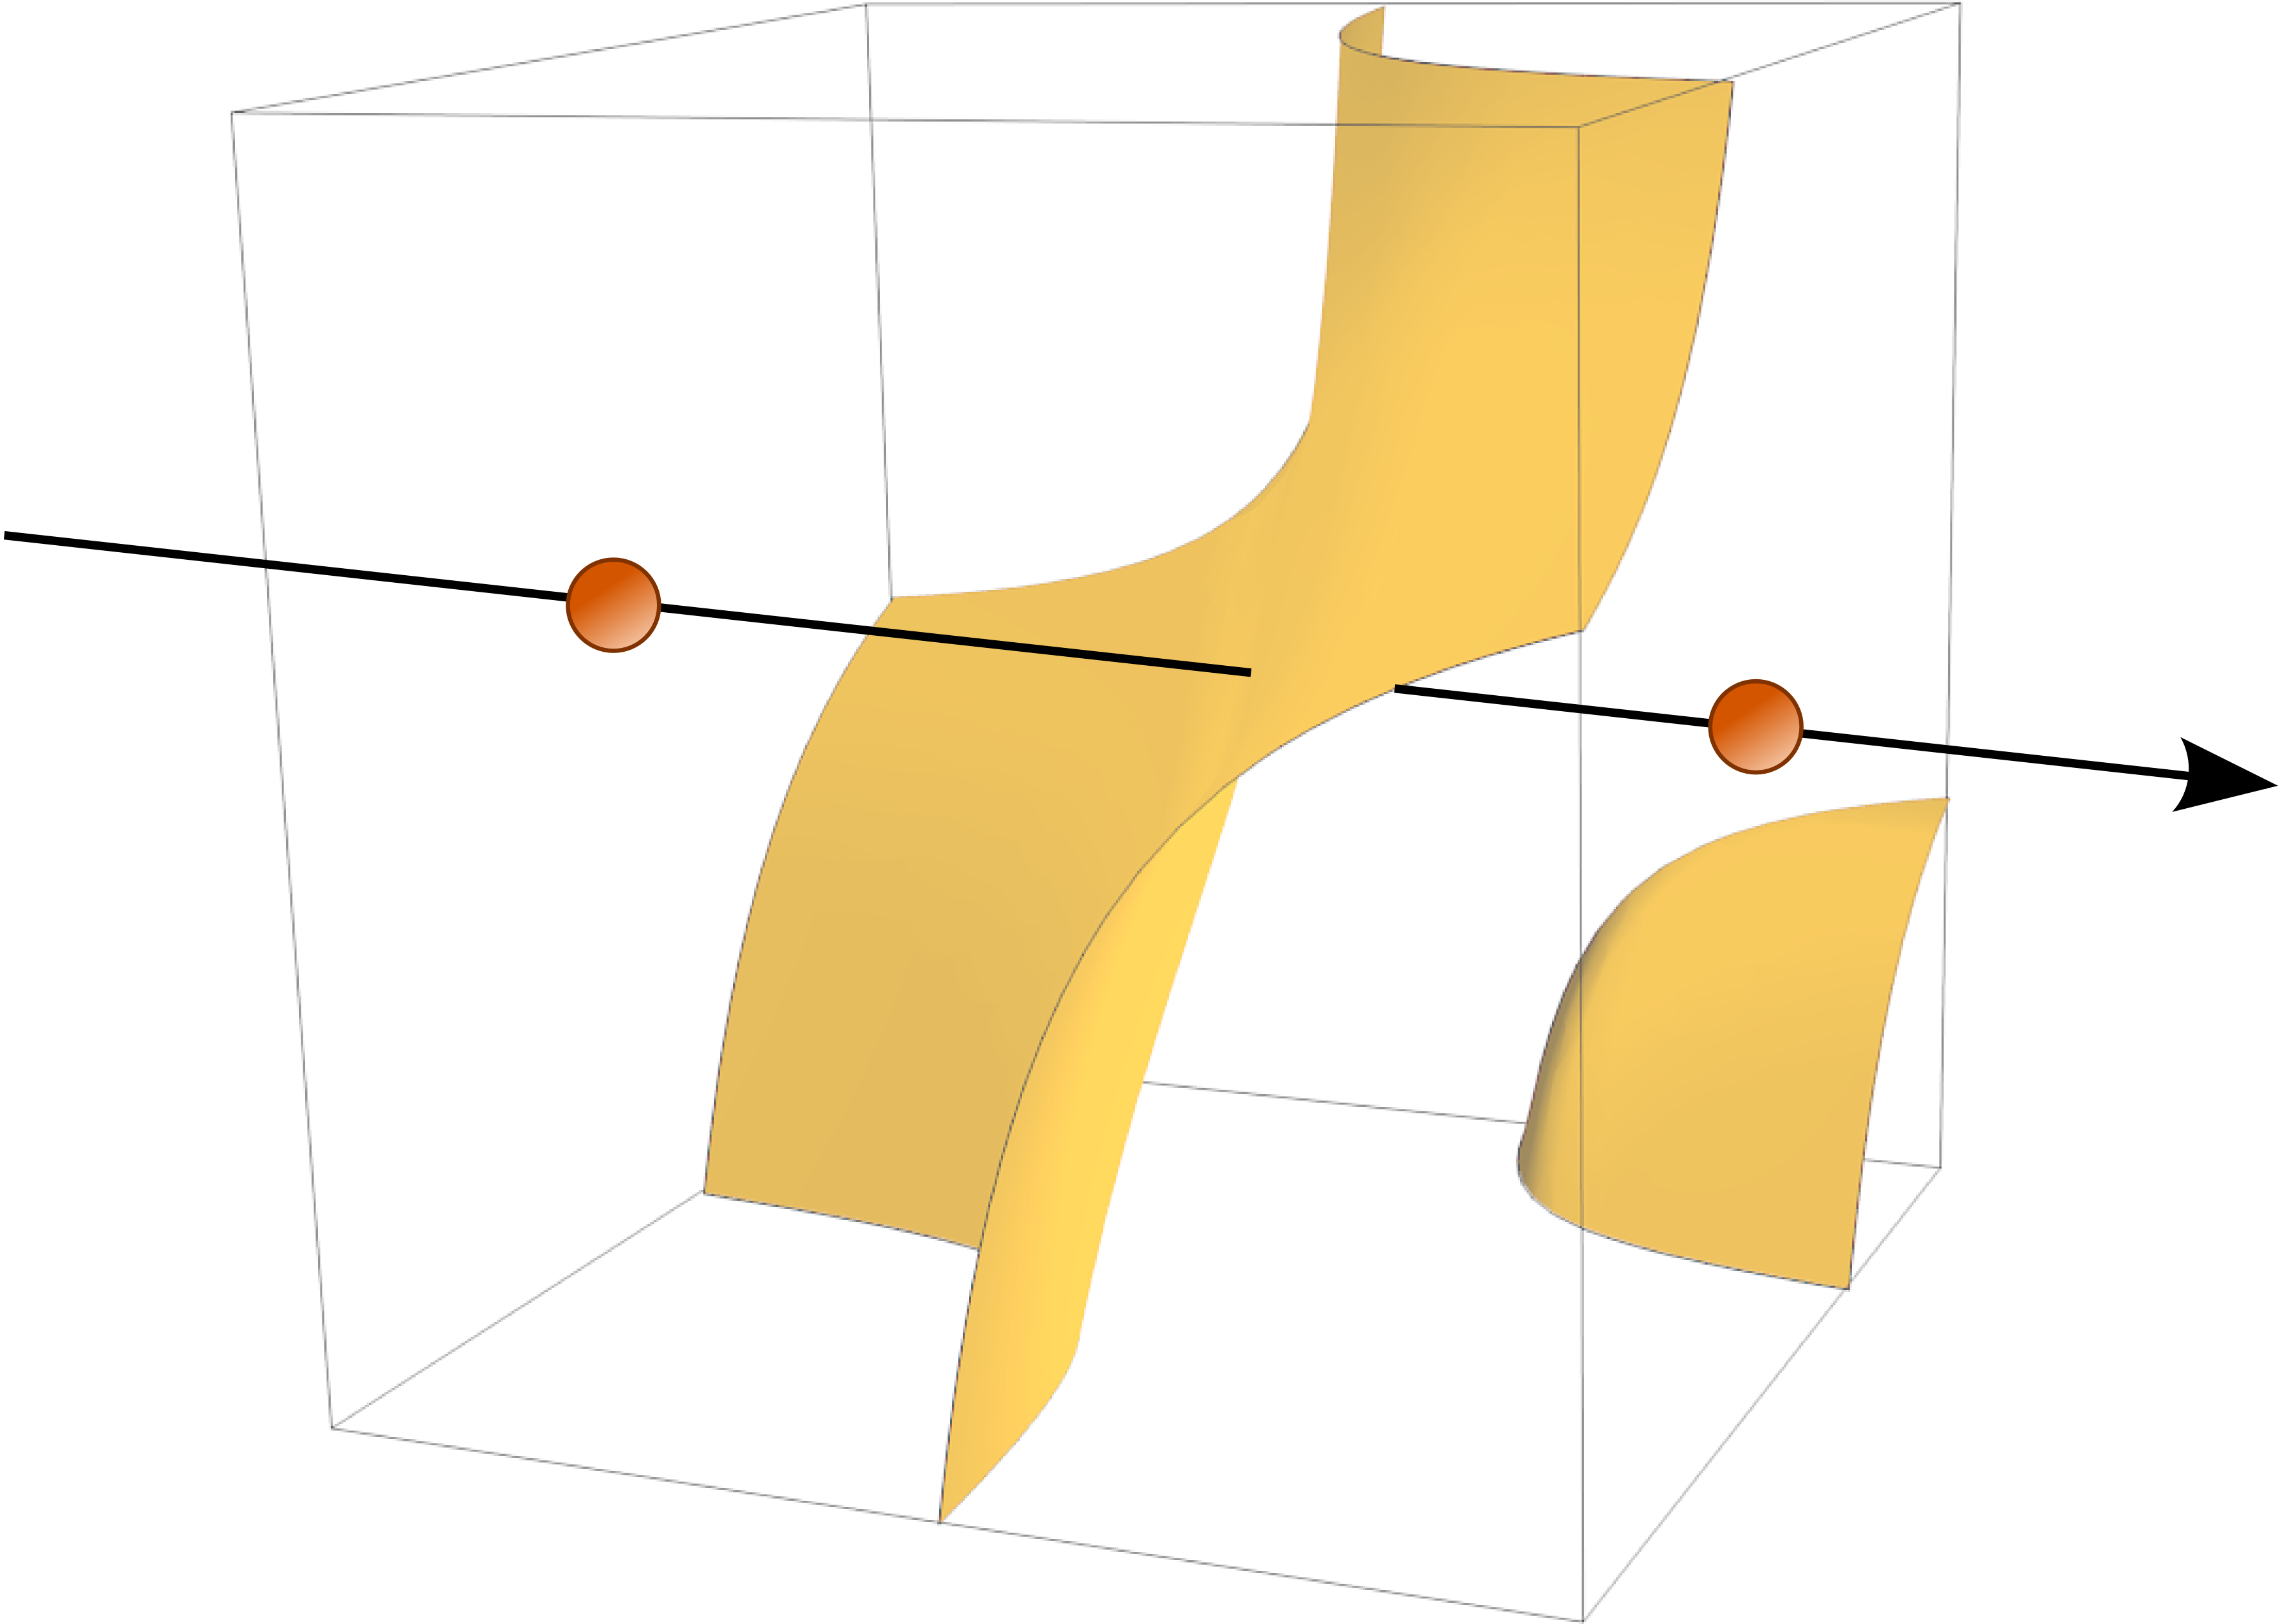
\includegraphics[width=0.24\linewidth]{chapter5/figures/ray-03.png}
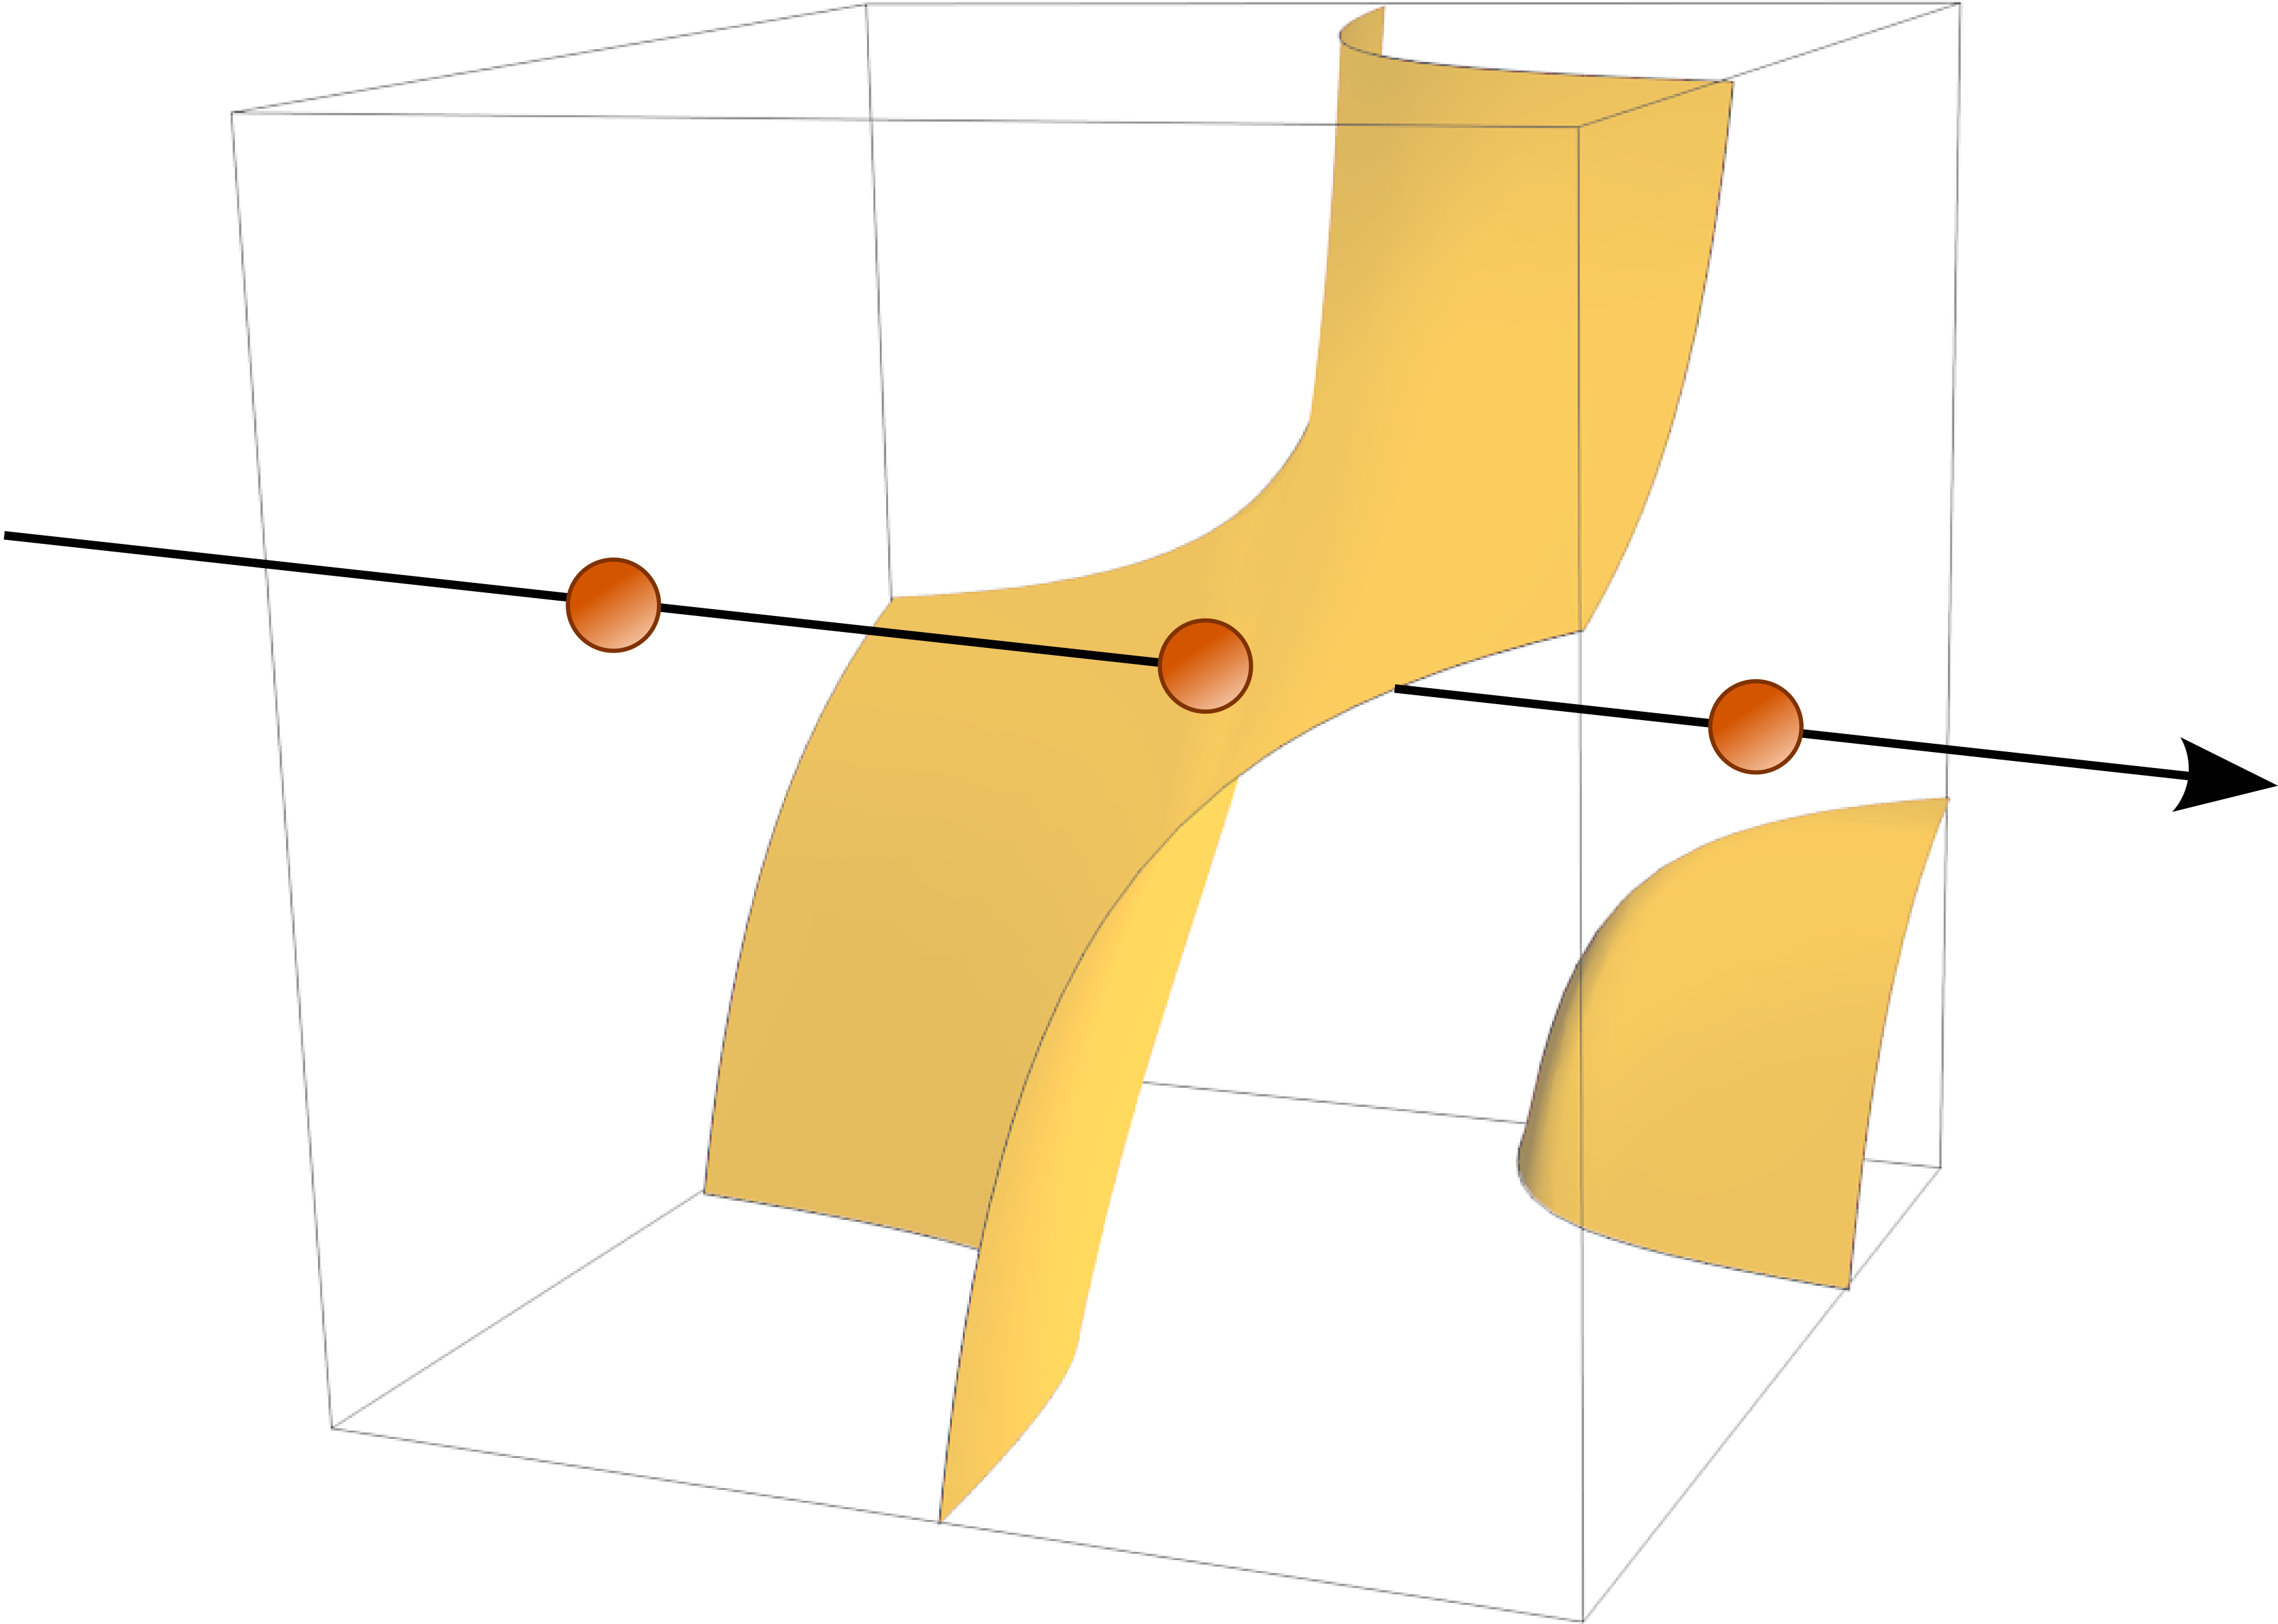
\includegraphics[width=0.24\linewidth]{chapter5/figures/ray-00.png}
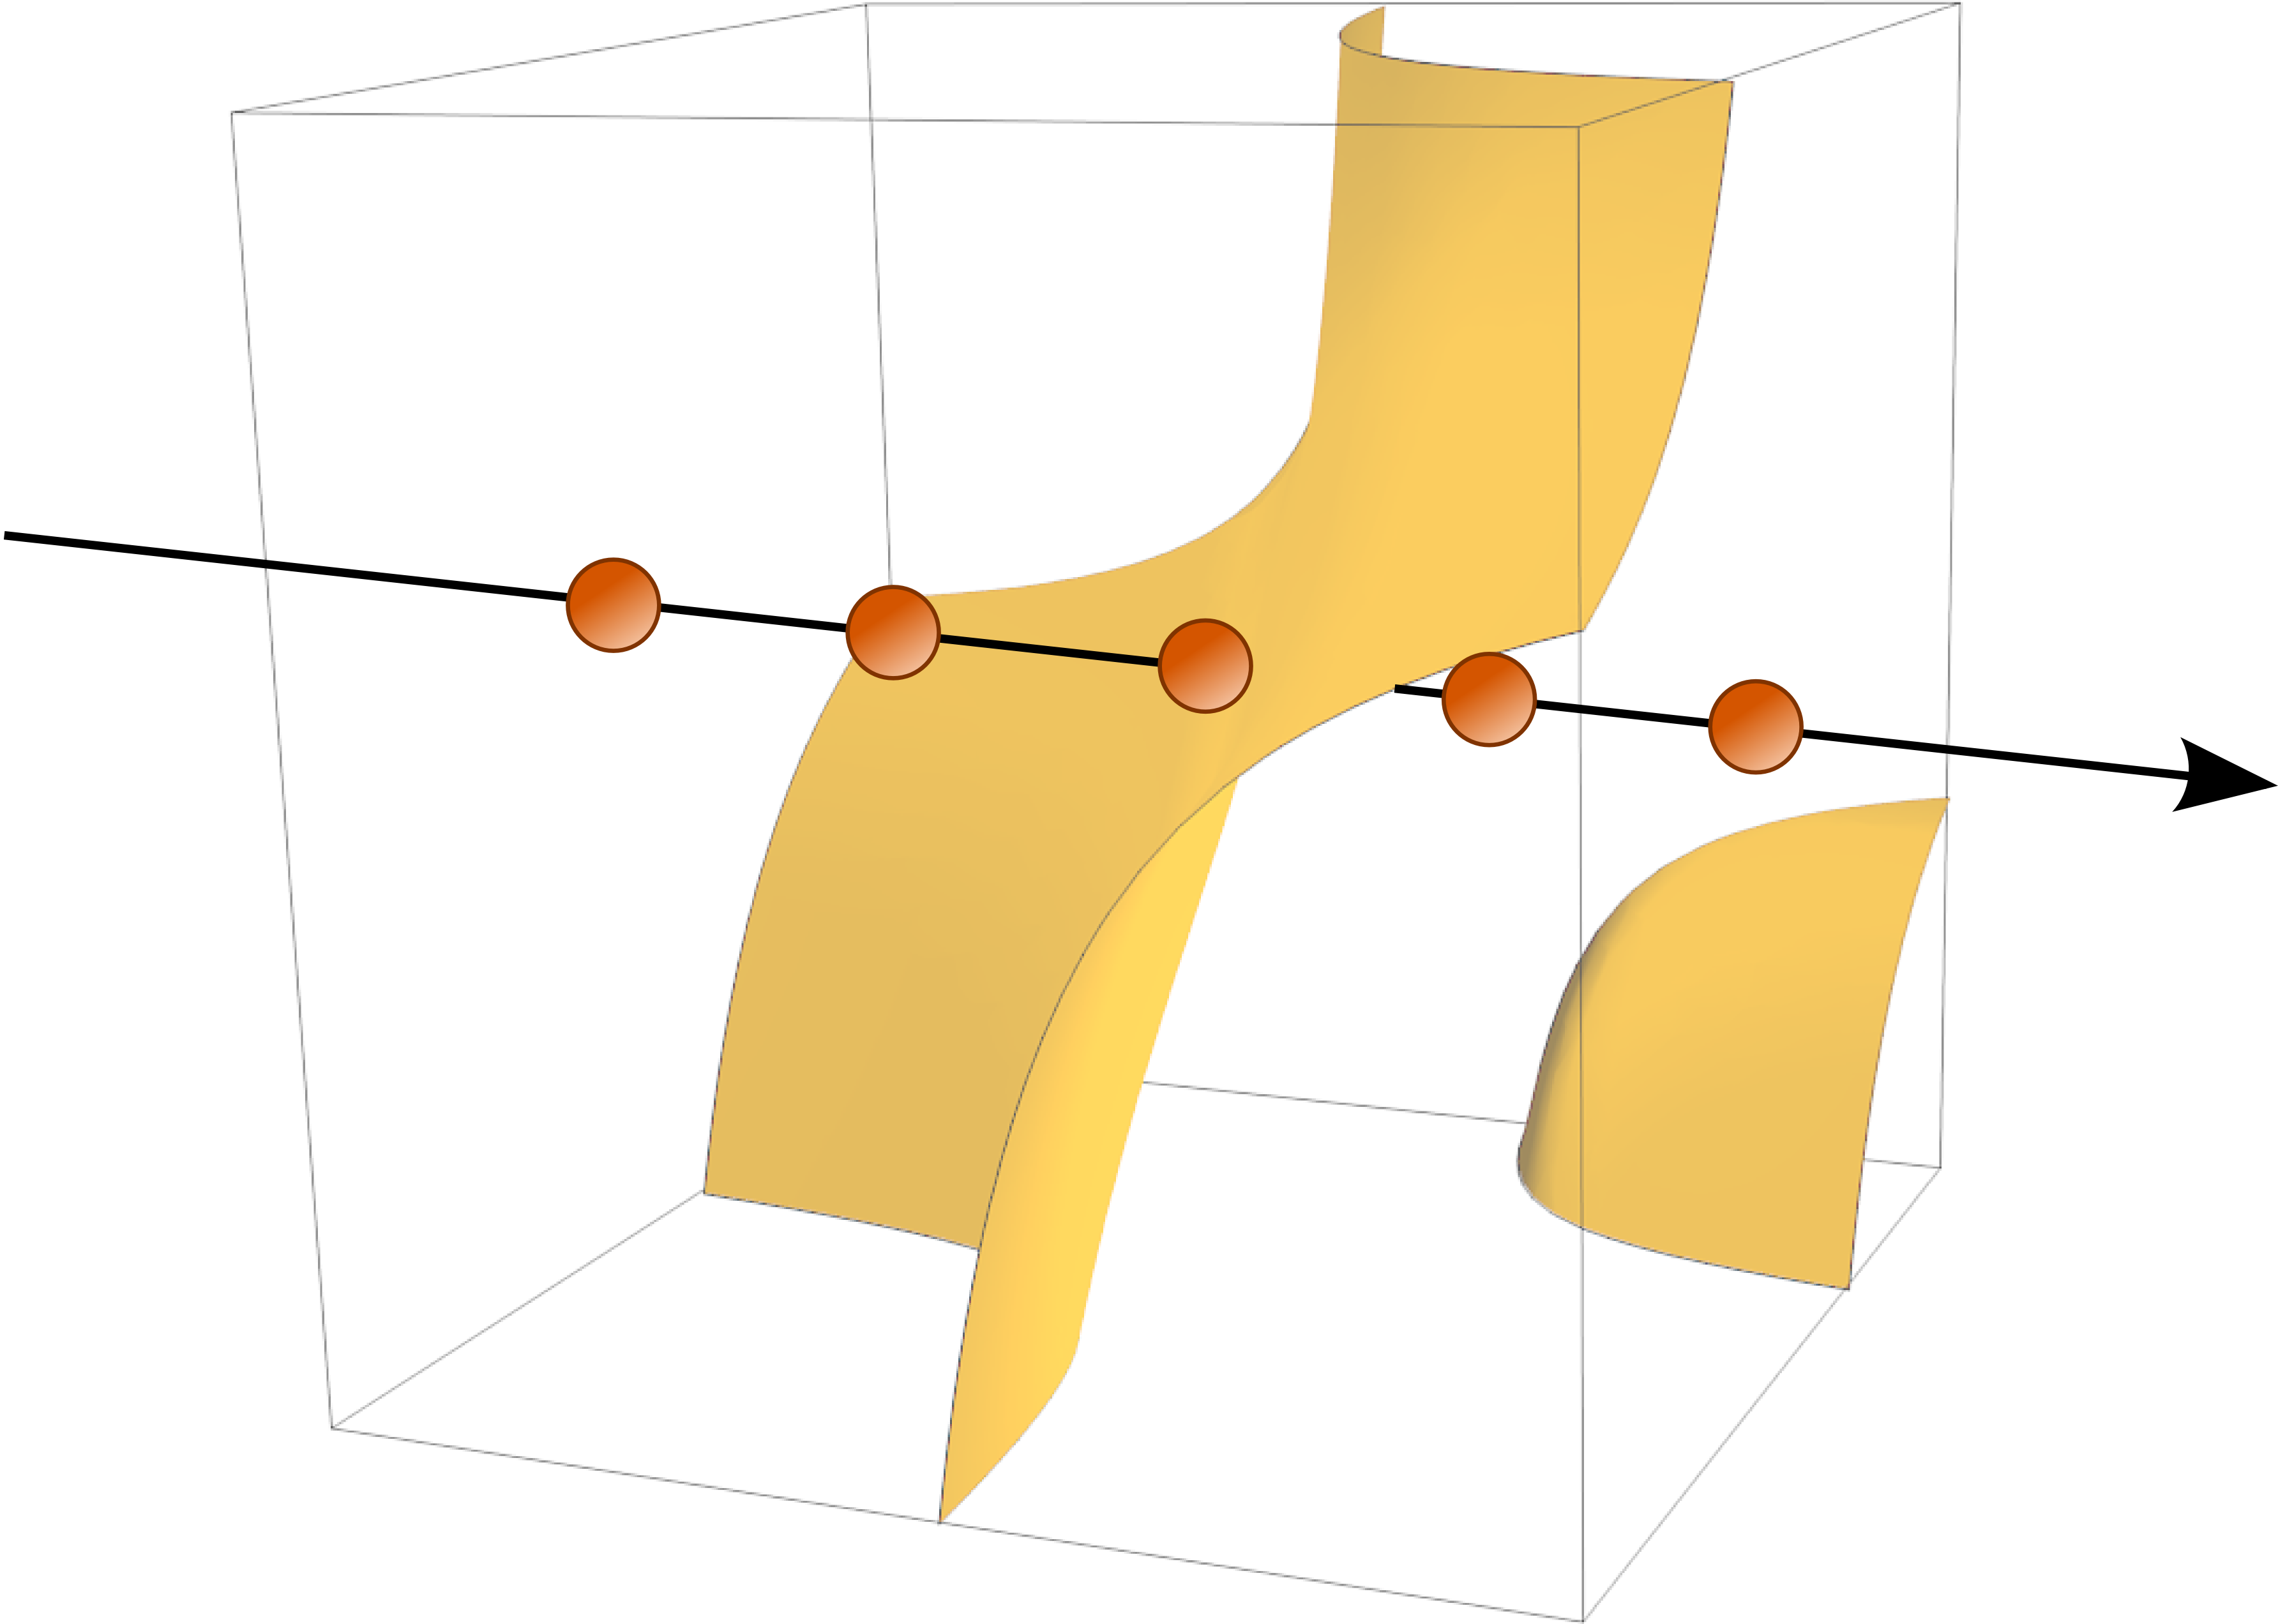
\includegraphics[width=0.24\linewidth]{chapter5/figures/ray-01.png}
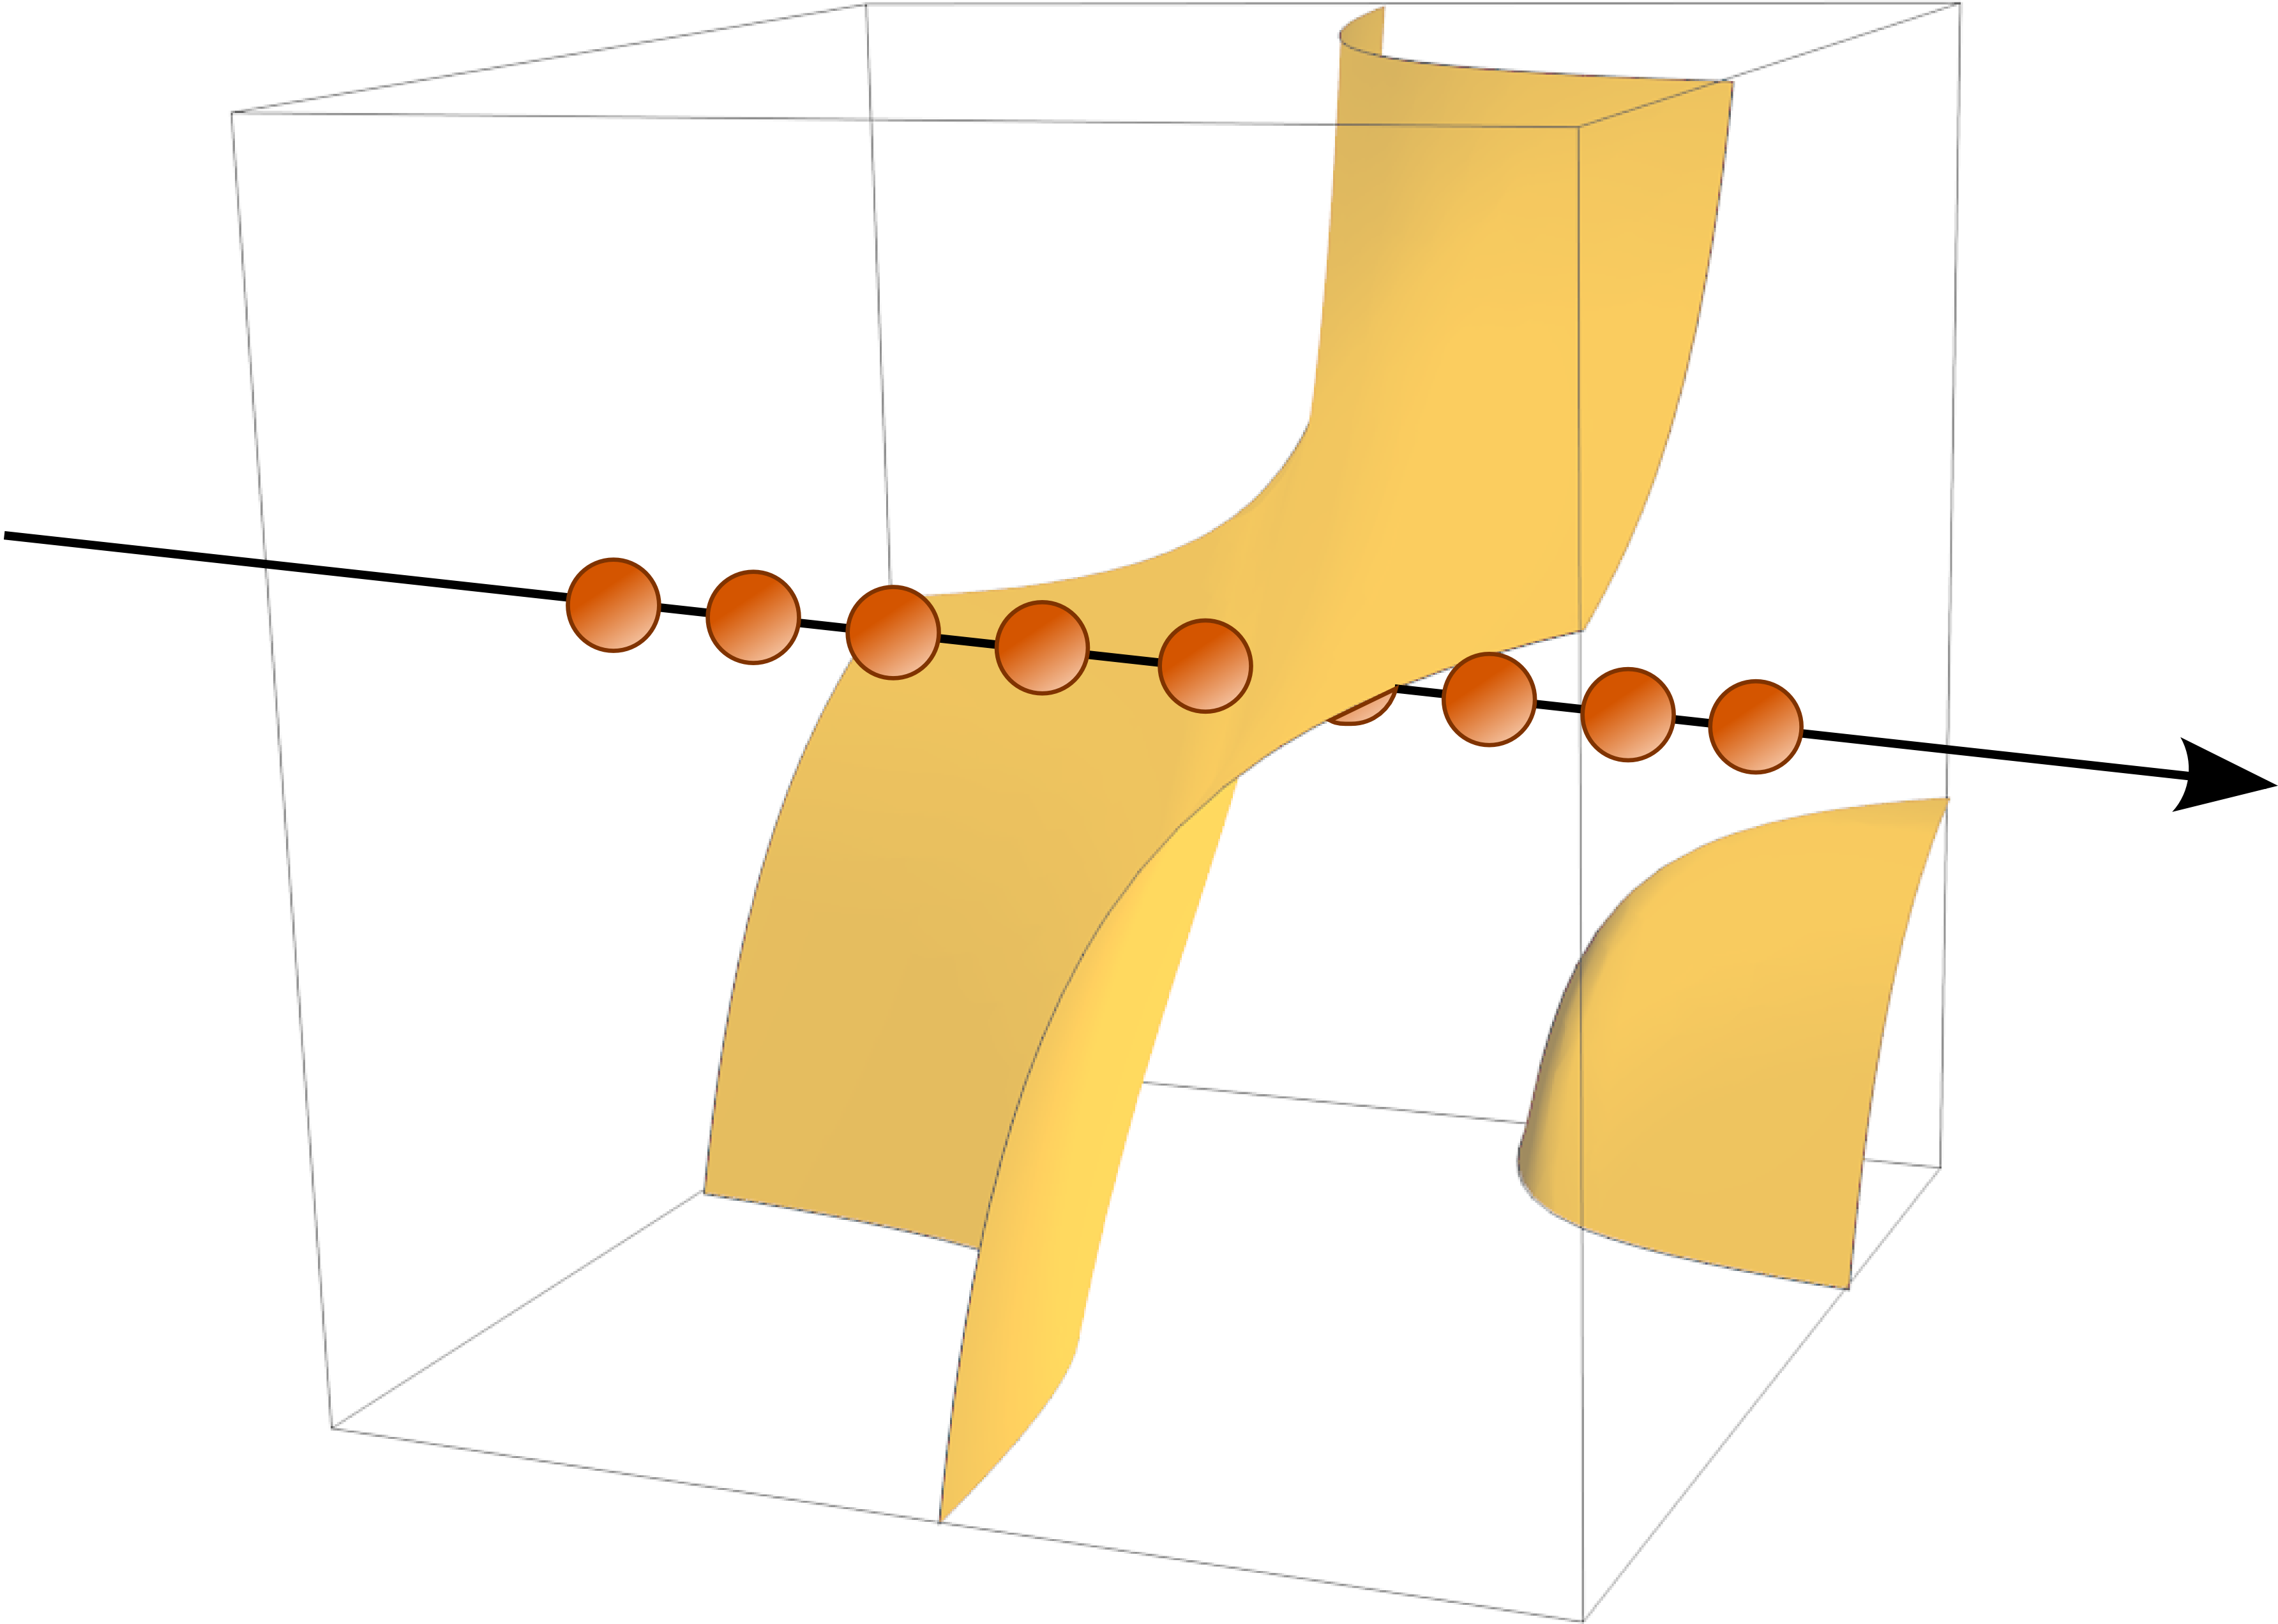
\includegraphics[width=0.24\linewidth]{chapter5/figures/ray-02.png}
\caption{\label{fig:stepsize_refinement} Step size refinement. The
  figure shows an isosurface of the trilinear function defined on the
  volume.}
\end{figure}
%
In this section, we are interested in the errors generated by
successive ray step refinements (see Figure
\ref{fig:stepsize_refinement}).  We first generate a sequence of
images $I_i$ using 
%a step size of $d_i = 1 / 2^i$.  
progressively smaller step size.
We then evaluate
the error $E_i$.  Equation~\eqref{eq:emission_absorption} is commonly
discretized using traditional Riemann sums for numerical integration:
\begin{equation}
\int_0^D f(s(\mathbf{x}(\lambda))) \mathrm{d}\lambda =
\sum_{i=0}^{n-1} f(s(\mathbf{x}(i d))) d + O(d),
\label{eq:rectangle-rule}
\end{equation}
where $n$ is the number of sub-intervals and $d = D  /
n$. The proof of linear convergence follows from Taylor expansion of
the integrand over small intervals $d$. 
%This implies that the errors involved in the Riemann sum decreases linearly with $d$. 
Other
methods are available and they provide different convergence rates.
For instance, the Trapezoid method is a 2nd order method on the integral
of $f$. 

In the case of the VRI, we approximate not only the outer integral but
also the integrand $T(s(\mathbf{x}(\lambda))) =
\exp\left(-\int_0^{\lambda} \tau(s(\mathbf{x}(\lambda')))
\mathrm{d}\lambda' \right)$. Moreover, $T$ requires two
approximations: $e^{t(\lambda)}$ and the inner integral. Before we derive the
convergence rate for the VRI, let us first evaluate the convergence of
$T$. Throughout the text, we assume that all transfer functions are
smooth, {\em i.e.,} $C(s), \tau(s) \in C^\infty$. Although
this is not the case in practice, this restriction is useful for convergence
evaluation and verification purposes.

\subsubsection{Approximation of $T(\lambda)$}
\label{appx:approximationT}

Let $T(\lambda) = T_\lambda = e^{-t(\lambda)}$, where $t(\lambda) = \int_0^{\lambda} \tau(\lambda')
\mathrm{d}\lambda'$, and $\lambda$ parameterizes a ray position. We
will first approximate $t(\lambda)$ and then $T(\lambda)$. Typically, the
integral is solved by using Riemann sums. 
In the following, $d = D / n$ is the ray sampling distance, 
$D$ is the ray length and $n$ is the number of sub-intervals along the ray:
\begin{eqnarray}
\int_0^{\lambda} \tau(\lambda') \mathrm{d}\lambda' & = &
\sum_{j=0}^{i-1}\tau(j d) d + O(d) \label{eq:order_integral}
\end{eqnarray}
%
where $\lambda = i d$. Using Equation \eqref{eq:order_integral}:
\begin{eqnarray}
T(\lambda) &=& \exp\left(-\int_0^{\lambda} \tau(\lambda')
\mathrm{d}\lambda'\right)\\ 
 & = & \exp\left(-\sum_{j=0}^{i-1}\tau(j d) d + O(d)\right)\\ 
& = & \left(\prod_{j=0}^{i-1}\exp\left(-\tau(j d) d\right)\right)
\exp\left(O(d)\right). 
\end{eqnarray}
%
Let us define $\tau_j = \tau(j d)$. We start with a Taylor expansion
of $\exp\left(O(d)\right)$:
%
\begin{eqnarray}
T_\lambda = \left(\prod_{j=0}^{i-1}\exp\left(-\tau_j
d\right)\right) \left(1 + O(d) \right).
\end{eqnarray}
In the equation above, we assume that high order terms are
negligible, and thus the dominant
error is $O(d)$:
\begin{eqnarray}
T_\lambda
& = & \left(\prod_{j=0}^{i-1}\exp\left(-\tau_j d\right)\right) \left(1 +
O(d)\right)\\
& = & \prod_{j=0}^{i-1}\exp\left(-\tau_j d\right) + \prod_{j=0}^{i-1}\exp\left(-\tau_j d\right)O(d)  \label{eq:m}
\end{eqnarray}

\paragraph*{Part I}
Let us focus on the second term in the right hand side of Equation \eqref{eq:m}. The first observation is that it contains only approximation errors, which means that we are  interested only in its asymptotic behavior. Let us expand it using first-order Taylor approximation and use the fact that  $\tau_j d = O(d)$: 
\begin{eqnarray}
\prod_{j=0}^{i-1}\left(1-O(d)\right)O(d) &=& \left(1+O(d)\right)^iO(d), \label{eq:error-q}
\end{eqnarray}
%
where the change in the sign is warranted because the goal is to determine the asymptotic behavior. For $i = 1$, only one step is necessary for computing the volume rendering integral along the ray, and the previous equation will exhibit linear convergence.  Nevertheless, in the general case, the numerical integration requires multiple steps, hence errors accumulate, and the convergence may change. Thus  we set $i = n$. Knowing that $(1 + O(d) )^{n} = O(1)$ (see Appendix \ref{sec:aux}) and inserting Equation \eqref{eq:error-q} into Equation \eqref{eq:m} we obtain:
\begin{eqnarray}
T_\lambda
& = & \prod_{j=0}^{i-1}\exp(-\tau_j d)  + O(d)O(1),
\end{eqnarray}
and the Taylor expansion of the first term yields:
\begin{eqnarray}
T_\lambda
& = & \prod_{j=0}^{i-1} \left(1 - \tau_jd + O(d^2)\right) + O(d).\label{eq:partial}
\end{eqnarray}

\paragraph*{Part II}
We now show that the first term on the right side of Equation \eqref{eq:partial}
also converges linearly with respect to $d$. In the course of this section, we omit the presence of the term $O(d)$ in Equation \eqref{eq:partial} for the sake of clarity. Let us define the set $K$ as the set of indices $j$ for which $1-\tau_j d = 0$. The size of $K$ is denoted as $|K| = k$. We also define $N$ as the set of indices $j$ for which $1-\tau_j d \neq 0$, and $|N|=i-k$.  
%
Equation \eqref{eq:partial} can be written as:
\begin{eqnarray}
T_\lambda
& = & \left( \prod_{j \in N}1 - \tau_jd + O(d^2) \right) \left( \prod_{j \in K}O(d^2) \right) \\
& = & \left( \prod_{j \in N}1 - \tau_jd + O(d^2) \right) O(d^{2k}).
\end{eqnarray}
Because $1-\tau_j d \neq 0$ for $j \in N$:
\begin{eqnarray}
T_\lambda
& = &\left( \prod_{j \in N} (1 - \tau_jd) \left(1 + \frac{O(d^2)}{1-\tau_j d} \right) \right) O(d^{2k})
\end{eqnarray}
From the definition of big O notation, $1/(1-\tau_j d) = O(1)$, hence:
\begin{eqnarray}
T_\lambda
& = &\left( \prod_{j \in N} (1 - \tau_jd) \left(1 + O(1)O(d^2) \right) \right) O(d^{2k})\\
& = &\left( \prod_{j \in N} (1 - \tau_jd) (1 +O(d^2) ) \right) O(d^{2k})\\
& = &\left( \prod_{j \in N} 1 - \tau_jd \right) (1 + O(d^2) )^{i-k} O(d^{2k}). \label{eq:k}
\end{eqnarray}

In real world implementation, $k \neq 0$ implies that at least one of the terms $1 - \tau_j d = 0$. Hence the code accumulating the value of $T$
\begin{verbatim}
T = T * (1 - t_j * d)
\end{verbatim}
will invariably return \texttt{T = 0}. This can also be seen in our theoretical analysis. For $k \neq 0$, the whole right hand side of Equation \eqref{eq:k} \emph{is} the approximation error. The larger $k$ is -- \emph{i.e.} the more zeroes in the product of Equation \eqref{eq:k} --  the faster the sequence converges to $0$ because of the $O(d^{2k})$ factor. So, when $k \neq 0$, we will have a high order approximation of $T_\lambda = 0$. Nevertheless, because we want to recover the approximation errors for the general case ($T_\lambda \neq 0$), we set $k = 0$ in Equation \eqref{eq:k}, and $i = n$ (for the same reasons as previously stated):
\begin{eqnarray}
T_\lambda
& = &\left( \prod_{j = 0}^{n-1} 1 - \tau_jd \right) (1 + O(d^2) )^{n}.
\end{eqnarray}
%
Using the fact that $(1 + O(d^2) )^{n} = 1 + O(d)$ and $(1 + O(d) )^{n} = O(1)$ (see Appendix \ref{sec:aux}):
\begin{eqnarray}
T_\lambda
& = &\left( \prod_{j = 0}^{n-1} 1 - \tau_jd \right) (1 + O(d))\\
& = &\left( \prod_{j = 0}^{n-1} 1 - \tau_jd \right)  +  O(d)\left( \prod_{j = 0}^{n-1} (1 + O(d)) \right) \\
& = &\left( \prod_{j = 0}^{n-1} 1 - \tau_jd \right)  +  O(d)(1 + O(d))^n \\
& = &\left( \prod_{j = 0}^{n-1} 1 - \tau_jd \right) + O(d)O(1) \\
& = &\left( \prod_{j = 0}^{n-1} 1 - \tau_jd \right) + O(d)
\end{eqnarray}
We finish our derivation by adding the previously omitted $O(d)$ term:
\begin{eqnarray}
T_\lambda
& = &\left( \prod_{j = 0}^{n-1} 1 - \tau_jd \right) + O(d) + O(d)\\
& = &\left( \prod_{j = 0}^{n-1} 1 - \tau_jd \right) + O(d)
\end{eqnarray}

\subsubsection{Approximation of the outer integral}

Let $\tilde{T_i}$ be the approximation of $T(\lambda_i)$. We write
$T(\lambda_i) = T_i = \tilde{T_i} + O(d)$, and $C_i = C(id)$.  
%
In typical volume rendering implementations, the outer integral is
also approximated using a Riemann sum. Thus:
\begin{eqnarray}
I(x,y) &=& \sum_{i=0} ^ {n-1} C(i d) \tau(i d) T_i d + O(d)\\
&=& \sum_{i=0}^{n-1} C_i \tau_i d \left(\tilde{T}_{i} + O(d)\right) + O(d)\\
&=& \sum_{i=0}^{n-1} C_i \tau_i \tilde{T}_{i} d + \sum_{i=0}^{n-1} C_i \tau_i d O(d) + O(d).
\end{eqnarray}
Because both $\tau_i$ and $C_i$ are bounded, one can write $C_i \tau_i d O(d) = O(d^2)$ and $\sum_i O(d^2) = n O(d^2) = \frac{D}{d}O(d^2) = O(d)$. The above equation can be re-written as:
\begin{eqnarray}
I(x,y)  &=& \sum_{i=0} ^ {n-1} C(i d) \tau(i d) d \tilde{T}_{i} + O(d).
\end{eqnarray}
We have now showed that the dominant error when considering step size
in the VRI is of order $O(d)$. In other words, when decreasing the step size by half, the
error should be reduced by half.


\begin{table}[b]
\normalsize
  \caption{Effects of the different integration methods.}
  \centering
  \begin{tabular}{c  r | c c }
  & & \multicolumn{2}{c}{Outer integral}\\
   &                & Riemann & Trapezoid  \\
    \hline
\multirow{3}{*}{\parbox{1cm}{Inner \mbox{integral}}} & Monte Carlo & $ O(d^{0.43}) $ & $ O(d^{0.58})$ \\
& Riemann      & $ O(d^{0.99}) $ & $ O(d^{0.98}) $ \\
&Trapezoid     & $ O(d^{1.01}) $ & $ O(d^{2.00})$ \\
    \hline  
  \end{tabular} 
  \label{table:orders} 
\end{table}

\subsubsection{Numerical integration techniques}

%The goal of this section is to mathematically evaluate the approximation errors involved in
% the classic discretization scheme of the VRI, namely, one that assumes that both the inner
  %and outer integral are approximated using Riemann sums. Naturally, one may also be interested
%  in the effects on the error when using other integration methods. 
The interplay between the approximation errors of the inner and outer integrals is non-trivial, and
  here we show a simple numerical example.  Table \ref{table:orders} shows the
  results of the effects of different integration methods for the inner and outer integrals along a 
  single ray. We simulate the integration along a single ray to compute these quantities
  numerically. For this experiment, we assume:
  $x \in [0,D]$, $\tau(s(x)) = \cos(s(x))$, $C(s(x)) = \sin(s(x))$, $s(x) = x$ 
  and thus the solution for the VRI is $I = 1-\exp{(-\sin(D))}(\sin(D)+1)$. 
  To evaluate the effects of the discretization errors of the integrals, 
  we further assume that $\exp(x)$ does not introduce errors.  
  The computation of the convergence rate is detailed in Section \ref{sec:convergence_analysis}. The results shown in Table \ref{table:orders} suggest
  that one needs to improve the accuracy of \emph{both} the inner and outer integrals to obtain
  high-order methods.  
  %In this chapter, we restrict ourselves to the classic discretization using Riemann sum 
  %for both inner and outer integrals. 
%  The results of this section will be used for the verification of 
%  widely used volume rendering packages, whichs implement the Riemann sum.

\subsection{Errors due to dataset refinement}
\label{sec:VerViaDatasetRefinement}

\begin{figure}[t]
\centering
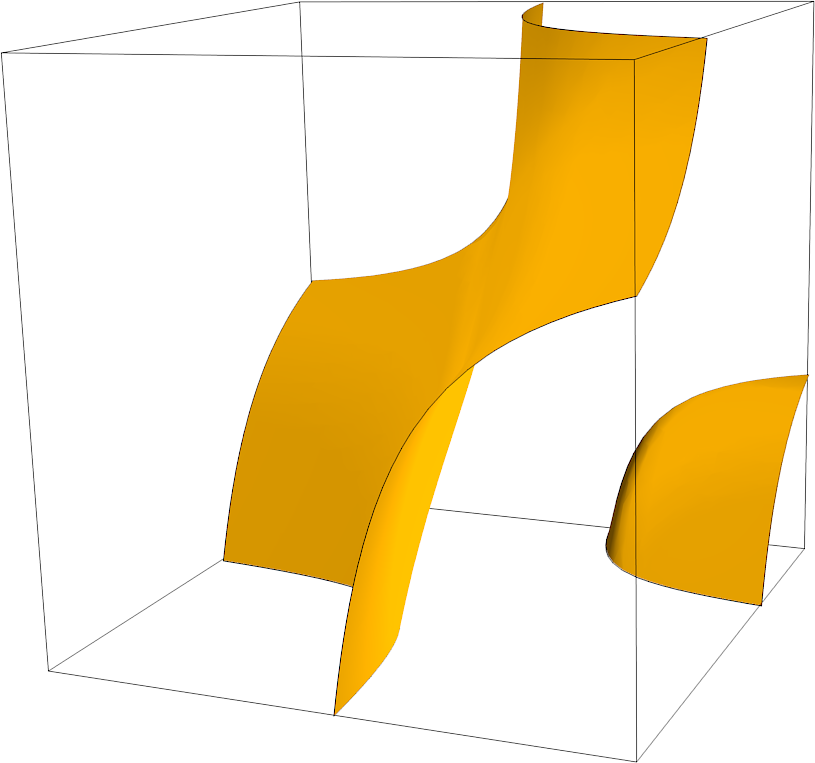
\includegraphics[width=0.24\linewidth]{chapter5/figures/grid_00.png}
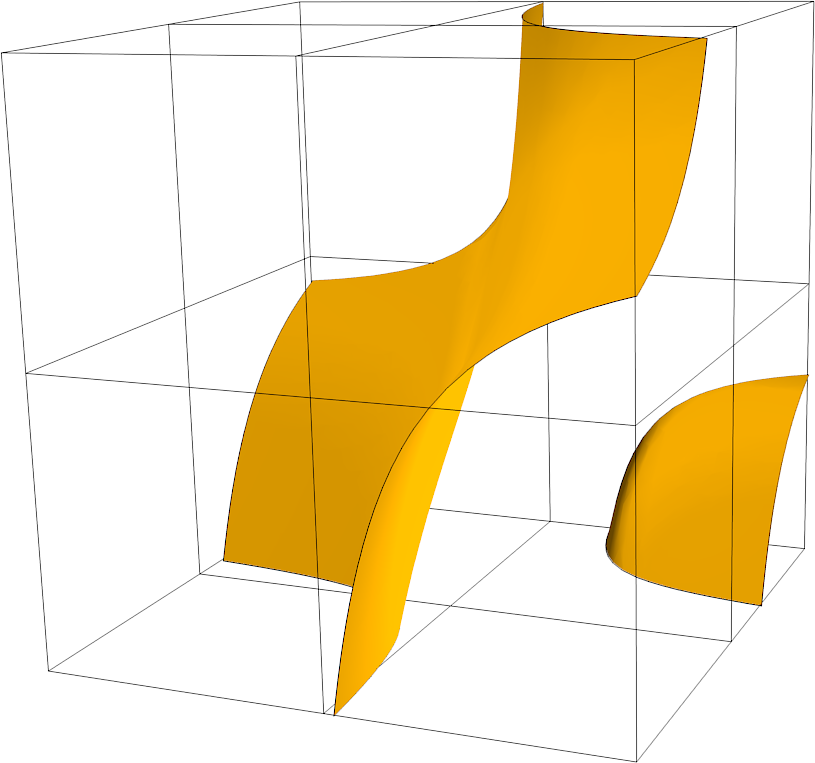
\includegraphics[width=0.24\linewidth]{chapter5/figures/grid_01.png}
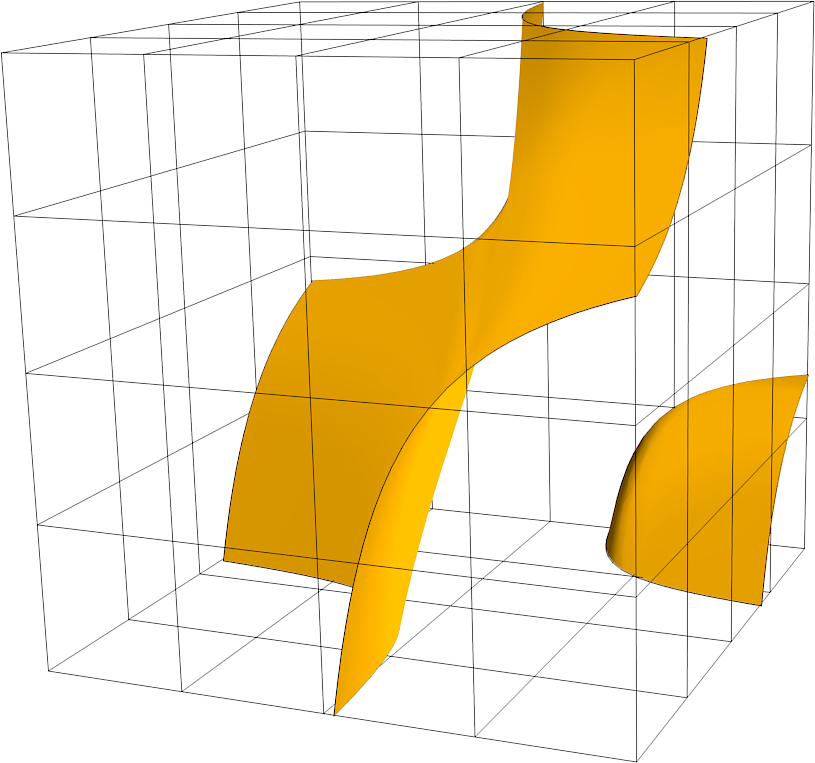
\includegraphics[width=0.24\linewidth]{chapter5/figures/grid_02.png}
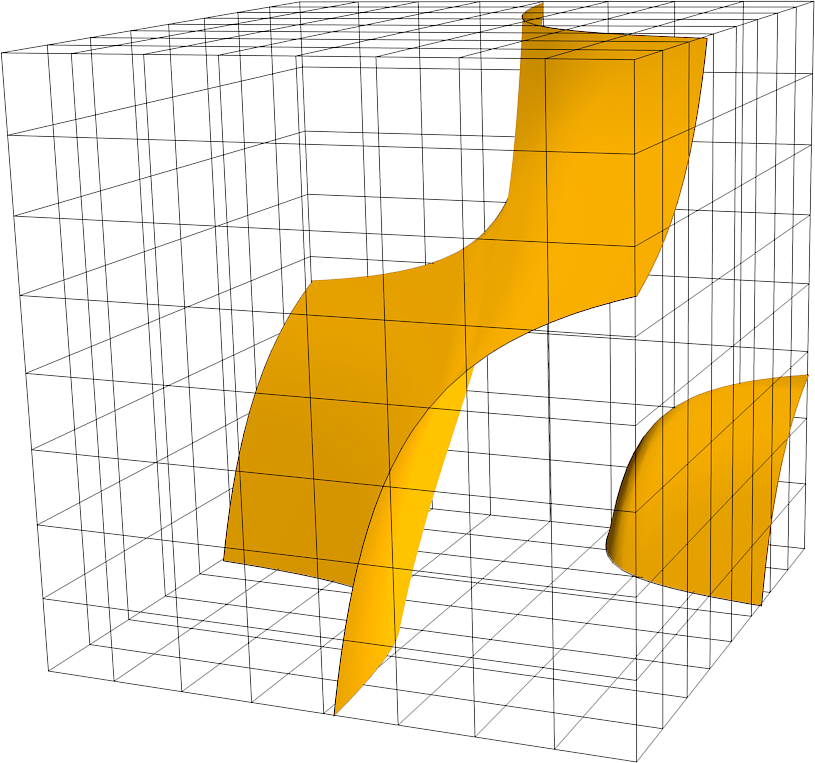
\includegraphics[width=0.24\linewidth]{chapter5/figures/grid_03.png}
\caption{\label{fig:dataset_refinement} Isosurface of a randomly generated 
   scalar field defined in different resolutions. The
  (piecewise) trilinear surface is the same regardless of the grid size.}
\end{figure}

%Errors due to the approximation of the scalar field can also propagate to
%the approximation of the VRI. Suppose that $s(\mathbf{x}) =
%\tilde{s}(\mathbf{x}) + O\left(N^{-u}\right)$, where $u$ is the order
%of accuracy of the reconstruction method, and $N$ is the number
%of points per dimension -- for instance, $\tilde{s}$ could be
%approximated using a radial basis function. The errors are then:
%\begin{eqnarray}
%I(x,y) &=& \sum_{i = 0} ^ {n - 1} C( \tilde{s}( \mathbf{x}_i) + O(
%N^{-u}) ) \tau( \tilde{s}( \mathbf{x}_i) + O(
%N^{-u}) )d \nonumber\\
%& & \qquad \tilde{T}(\tilde{s}(\mathbf{x}_i) +
%O(N^{-u})) + O(d).
%\end{eqnarray}
%An interesting case, which is the focus of this paper, occurs when
%the approximation $\tilde{s}(\mathbf{x})$ \emph{does not} introduce
%any error that is a function of $N$, {\em i.e.}, $s(\mathbf{x}) =
%\tilde{s}(\mathbf{x})$ (see Figure \ref{fig:dataset_refinement}). In
%this case, no matter what the refinement level $N$, the error is dominated
%by $O(d)$ (due step size refinement), and not by
%$O(N^{-u})$. For volume rendering, this can be easily achieved by
%assuming that the unknown  scalar field $s(\mathbf{x})$ is as a (piecewise) trilinear function:
%\begin{eqnarray}
%s(\mathbf{x}) = a xyz + b xy + c xz + d yz + e x + f y +g z + h.
%\end{eqnarray}
%%
%The sampling process on a $2 \times 2 \times 2$ or $N \times N \times
%N$ grid does not introduce errors dependent on $N$ because, typically, the trilinear
%interpolant is used for reconstruction of
%the scalar field. For dataset refinement, we restrict ourselves to the case of piecewise trilinear
%interpolants. This is a valid assumption for verification 
%purposes because in this chapter we are not  interested in the quality of the 
%approximation of the unknown scalar field but  instead we need
% a property that can be tested under the outlined assumptions (and the
% piecewise trilinear field provides us such a property). Moreover, the software packages tested in this chapter, 
% and many more, also use a trilinear interpolant.  If other interpolants are used, there may be an 
%approximation error due to grid size. 

For the purposes of this chapter, we assume that no additional 
errors will be created during the refinement of the scalar field. 
Hence, we need to find an interpolation function, that fulfills the 
so called two-scaling property. Fortunately, B-splines fulfill the 
two-scale property~\cite{799930} and we will pick the linear B-spline, 
which results in the well-known tri-linear interpolator. Care must 
be taking on the refinement step. In this chapter we will pick a 
refinement factor of two, which simplifies to a simple averaging of 
the nearest neighbours. The errors introduced so far remain 
unchanged:

%Assuming a piecewise trilinear scalar field, for the same scalar field defined in
%datasets with different resolutions one should obtain the same
%images. We generate these datasets by successive upsampling of an $N
%\times N \times N$ piecewise-trilinear field. In the upsampling
%process, we keep the original nodes. The scalar value at new nodes
%does not change the original scalar field because they are
%interpolated directly using a trilinear interpolant. 
%
%The error is then constant, and we obtain zeroth-order convergence for
%dataset refinement. In other words, as the size of the dataset
%changes, no error is introduced. Here we assume a trilinear
%interpolant inside the cubes, and the new nodes of the refined grid
%will be interpolated with the same interpolant. The dominant error is
%then similar as previously stated:
%
\begin{eqnarray}
I(x,y) = \sum_{i = 0} ^ {n - 1} C( \tilde{s}( \mathbf{x}_i)) \tau(
\tilde{s}( \mathbf{x}_i)) d \tilde{T}(\tilde{s}(\mathbf{x}_i)) + O(d). \label{eq:datasetsize}
\end{eqnarray}

%In practice, high-resolution grids are used to mitigate errors. Here,
%on the other hand, we do not introduce any additional errors.
%%deliberately choose not to change the errors involved in the
%%approximation. 
%Although this may seem odd, it makes
%sense from the point of view of verification because the goal is to
%verify code correctness using Equation \eqref{eq:datasetsize}. For
%dataset size refinement, 
%the important property to be preserved, 
%under the assumptions outlined,
%is that the code under verification must not
%generate different images. As we will show later, this test helped us
%find bugs in one of the tested codes (cf. Section \ref{chap5:sec:results}). %the abbreviation has a single period after it ("cf.", not "c.f.") because it represents a shortening of the single word confer

The fact that no error due to grid resolution is introduced 
into Equation \eqref{eq:datasetsize} can
be interpreted as an ``infinity order of convergence'' on the grid
size $m$, $O(m^{-\infty})$; {\em i.e.}, an instantaneous convergence to zero error.
%
Nevertheless, Equation \eqref{eq:datasetsize} still contains an error due 
to ray sampling $O(d)$, and others  not considered in this chapter 
(such as rounding errors, finite precision, etc.).  
These fixed error sources will be revealed in the approximation 
of the VRI and remain (mostly) unchanged when refining dataset size.
Hence, even though no errors are introduced, one still expect
constant error on the approximation of the VRI, mainly due to the $O(d)$ term. 
Thus, from now on, we will say that the expected order of accuracy for
the grid size \emph{test} is constant, even though the convergence rate \emph{with respect to}
$m$ is $O(m^{-\infty})$.

\subsection{Errors due to pixel size refinement}
\label{sec:VerViaPixelRefinement}

\begin{figure}[t]
\centering
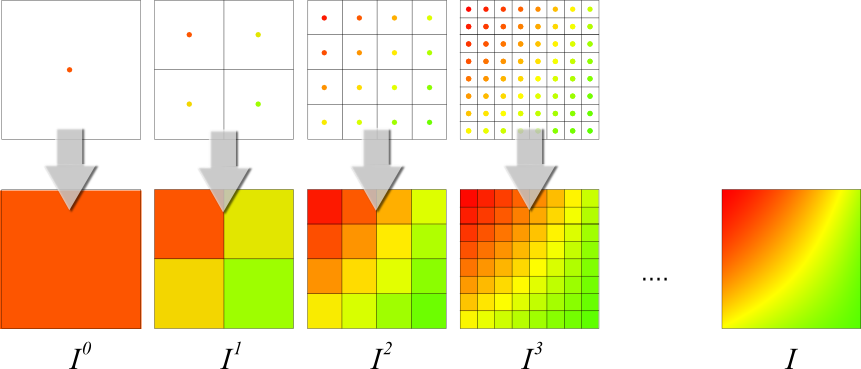
\includegraphics[width=0.95\linewidth]{chapter5/figures/pixel-size-convergence.png}
\caption{\label{fig:pixel_size_refinement} Pixel refinement. Typically, the VRI is evaluated
only at pixel centers (top). The value at the center is then interpolated in the domain defined by the pixel size (bottom) using
nearest-neighbor interpolation to obtain $\tilde{I}^i$. In a correct
implementation, as $i$ increases, $\tilde{I}^i$ approaches the true
solution $I$.}
\end{figure}

The final source of errors we investigate comes from the finite
number of rays sent into the image. One way of quantifying these errors
is to create a sequence of images of progressively higher resolution,
and then examine the supremum of the difference between values of the
finite approximations of the volume-rendered image and the true
solution.  In this section, we assume that the derivatives along image axes of
the volume rendering integral exist.

Denote the true volume-rendered image as $I(x,y)$. The approximation is
constructed by sampling $I(x,y)$ in a finite subset of the domain (in
our case, a square lattice of increasing resolution). At a level of
detail $j$, $\tilde{I}^j(x,y)$ denotes the nearest-neighbor
interpolation of the sampled values, and the error is measured as
$E_j = \sup_{(x,y) \in [0,1]^2} |I(x,y) - \tilde{I}^j(x,y)|$. Effectively, this 
procedure assigns to the entire square pixel the value sampled in its
center, but evaluates the error \emph{over the entirety of the pixel values}.
Figure \ref{fig:pixel_size_refinement} illustrates the
process.

We use the notation $I = I(x,y)$, $I^j_i = I^j(x_i, y_i)$, and $\delta_i =
(x, y) - (x_i, y_i)$. In what follows, the Taylor expansion assumes a fixed level of detail $j$. 
We omit the superscript $j$ for the sake of clarity. Let us write
 the values of $I$ as a Taylor series expansion ($\mathbf{H}_i = 
 \mathbf{H}(x_i, y_i)$ and is the Hessian and $I_i^x$ and $I_i^y$ 
 are the partial derivatives of $I_i$ at $(x_i, y_i)$):
\begin{eqnarray}
I &=& \tilde{I}_i + \nabla I_i^T \delta_i + \frac{1}{2}\delta_i^T \mathbf{H}_i
\delta_i + \cdots \\
  &=& \tilde{I}_i + O(\nabla I_i^T \delta_i)\\
  &=& \tilde{I}_i + O( (I_i^x, I_i^y)^T (x - x_i, y - y_i)),
\end{eqnarray}
$\tilde{I}_i$ is a nearest-neighbor reconstruction from a square
lattice for the pixel $(x_i, y_i)$ and at a given level $j$. In the regime where the Hessian terms are negligible, the
dominant errors (and hence the supremum of the difference) occur 
when $(x - x_i, y - y_i) = (h, h)$, where $h$ is half the pixel size.
Thus: 
\begin{eqnarray}
I &=& I_i + O(h)\\
&=& \sum_{i = 0} ^ {n - 1} C (\tilde{s}(\mathbf{x}_i))\tau(
\tilde{s}( \mathbf{x}_i)) \tilde{T}d(\tilde{s}(\mathbf{x}_i))) +\nonumber\\
&& ~~~~~~ + O(h) + O(d). \label{eq:complete}
\end{eqnarray}
As can be seen, the error in pixel approximation decays linearly with the pixel
size. Equation~\eqref{eq:complete} contains all the errors we use for
verification purposes and it will be the base for our analysis in
Section~\ref{sec:convergence_analysis}.

In practice, often the final image is not
%represented by 
a smooth function. However, our goal is not to provide a
characterization of discretization errors that can be used in any
setting, but instead one that can be used for
verification purposes. Therefore, 
to use the analysis outlined above,
%when using these approximation errors, 
one must manufacture scalar field and transfer functions which yield a smooth function (cf. Section~\ref{chap5:sec:results}).

%The discretization due to pixel size refinement is similar to the
%convergence of 2D regular grids. 
%% . Here, we assume that the solution to the volume rendering
%% integral is smooth in the whole image.

%% In order to account for the errors that are due to pixel size
%% refinement, we first write the approximation of the VRI as a Taylor
%% expansion. We use the notation $I = I(x,y)$, $I_i = I(x_i,
%% y_i)$, and $\delta_i = (x, y) - (x_i, y_i)$:
%% \begin{eqnarray}
%% I &=& I_i + \nabla I_i^T \delta_i + \frac{1}{2}\delta_i^T \mathbf{H}_i
%% \delta_i + \cdots
%% \end{eqnarray}
%% where $\mathbf{H}_i = \mathbf{H}(x_i, y_i)$ is the Hessian at $(x_i, y_i)$. Note that
%% $I_i$ are the (exact) values at the pixels $(x_i, y_i)$. This implies
%% that pixel refinement is a Taylor approximation up to the first
%% term. Therefore, the approximation is:
%% \begin{eqnarray}
%% I &=& I_i + O(\nabla I_i^T \delta_i)\\
%%   &=& I_i + O( (I_i^x, I_i^y)^T (x - x_i, y - y_i)).
%% \end{eqnarray}
%% The dominant error occurs when $(x - x_i, y - y_i) = (h, h)$, where
%% $h$ is the pixel size. Thus: 
%% \begin{eqnarray}
%% I &=& I_i + O(h)\\
%% &=& \sum_{i = 0} ^ {n - 1} C (\tilde{s}(\mathbf{x}_i))\tau(
%% \tilde{s}( \mathbf{x}_i)) \tilde{T}d(\tilde{s}(\mathbf{x}_i))) +\nonumber\\
%% && ~~~~~~ + O(h) + O(d). \label{eq:complete}
%% \end{eqnarray}
%% %
%% Thus, the error in pixel approximation decays linearly with the pixel
%% size. Equation \eqref{eq:complete} contains all the errors we use for
%% verification purposes and it will be the base for our analysis in the
%% Section \ref{sec:convergence_analysis}.

%% In practice, often the final image is not
%% %represented by 
%% a smooth function since discontinuities may arise due to several
%% different sources. Nevertheless, our goal is not to provide a
%% characterization of discretization errors that can be used in any
%% setting, but instead one that can be subject to
%% verification. Therefore, 
%% under the verification technique outlined above,
%% %when using these approximation errors, 
%% one must
%% manufacture a scalar field and transfer functions that yield a smooth function (cf. Section \ref{chap5:sec:results}).

%% \subsection{Discretization error conclusion}
%% \label{sec:discretization-error-conclusion}

%% Our algorithm builds upon the mathematical derivation of the 
%% discretization error for three different parameters of Equation 
%% \eqref{eq:volume-rendering-equation}, which we derived in the previous subsections. 
%% More specifically, we are interested in analyzing the discretization errors  
%% for the three parameters step size ($d$), data resolution ($n$) and pixel size ($h$). 
%% To conclude the results of these derivations we will 
%% now restate Equation \eqref{eq:complete} and explain the results.
%% \begin{eqnarray}
%% I(x,y) = \sum_{i = 0} ^ {n - 1} c (\tilde{s}(\mathbf{x}_i))\tau(
%% \tilde{s}( \mathbf{x}_i))d \tilde{T}(\tilde{s}(\mathbf{x}_i))) +
%% O(h) + O(d)
%% \end{eqnarray}
%% In the above equation we will first concentrate on the step size, derived in Section \ref{sec:StepSizeMathematicalDerivation},
%% which has discretization error of order $O(d)$.
%% This means that, when decreasing the step size by half, the
%% error should be reduced by half.

%% As discussed in Section \ref{sec:VerViaDatasetRefinement} and in Figure \ref{fig:dataset_refinement}
%% no error is introduced if
%% trilinear interpolation is used to increase the data resolution.
%% %we can see that the discretization error is zero. This might seem counterintuitive at first. 
%% %However, the reason for this is that we assume that the scalar field does not change as we change 
%% %the resolution of the dataset, which is discussed in more details in section \ref{sec:VerViaDatasetRefinement}
%% %and can be seen in Figure \ref{fig:dataset_refinement}. 
%% This means that, as one varies the resolution of the dataset, the resulting  
%% image should not change.

%% Pixel size error, derived in Section \ref{sec:VerViaPixelRefinement},
%% also converges linearly.  Thus, decreasing the pixel size by half then the error should also be reduce by half.

%% Removed for the sake of space
%%We have now concluded how the discretization error should behave when changing
%%three different parameters in the volume rendering equation. This is the foundation
%%of our method and will be used in section \ref{sec:convergence_analysis} to create 
%%a simple method which compares the derived discretization error with that of an implementation 
%%to verify if it behaves as expected. 
 
%% \subsection{Alternative approximation methods}

%% To make the derivations easier to follow, we chose to make some
%% assumptions when discretizing the VRI equation, such as Riemann sum
%% and trilinear interpolation.  Although these assumptions may be
%% common, not all implementations use them which is why we provide an
%% additional derivation in the appendix. The derivation in the appendix
%% derives the behavior of the discretization errors of the VRI without
%% assuming any particular approximation method. This means that the
%% potential users of our method can then derive the error behavior of
%% their particular implementations from the appendix and still use the
%% methods presented later to verify their implementations.


\section{Convergence computation}
\label{sec:convergence_analysis}

The heart of our method is the evaluation of the discretization
errors. Once we have the discretization errors, we can evaluate the
order-of-accuracy and convergence rate.  The error computation and
analysis will proceed differently depending on whether an analytical
solution for the VRI is available or not. We highlight that previous
frameworks for verification of visualization algorithms could benefit
from the fact that analytical solutions can be easily constructed
\cite{etiene:tvcg:2009}. For the case of VRI, this is no longer true and
therefore we should not count only on known solutions.  We describe
two ways in which to proceed with the convergence analysis. First, we
will show how to calculate errors using a known solution, and then how
to do so using an unknown solution.

\subsection{Numerical errors using a known solution}

When a solution $F(x,y)$ for the VRI is known, the procedure is equivalent
to the Method of Manufactured Solutions~\cite{babuska04}.  In the
previous section, we have shown that the 
solution $F$ can be written as:
\begin{eqnarray}
F(x,y) = I(x,y) + O(r^k) = I(x,y) + \beta r^k + \text{HOT},
\end{eqnarray}
where $I$ is the approximated image, $r$ is the discretization parameter (step size, grid size, or
pixel size) and $\beta \in \mathbb{R}$ is a constant, multiplicative
factor that is not a function of the dataset. An important assumption
is that HOT, or ``higher order terms'', are small enough so that it
does not affect the convergence of order $k \in \mathbb{R}$, {\em i.e.}, high order
derivatives of $F$ must have negligible impact in the asymptotic
convergence of $I$~\cite{Roy2005}. 
This formulation implies that not all solutions
$F$ are suitable for verification purposes, only those for which HOT is
negligible. In addition, integration methods whose approximation errors 
cannot be written as shown,
cannot be compared by only evaluating $k$, as we propose next. 
The expected value of $k$ for the cases of step size and pixel size 
convergence is $k = 1$ whereas $k = 0$ for grid size. 
This implies that the pixel intensity
converges to the true solution with ``speed'' determined by $k$ and
thus the error can be written as:
\begin{equation}
e(x,y) = I(x,y) - F(x,y) \approx \beta r^k.
\end{equation}
One can evaluate the convergence for all pixels in the image using
$L_2$, $L_\infty$, or other norms. Henceforth, we adopt the $L_\infty$
because it provides a rigorous way of evaluating errors: it tells us
that the maximum image error should decay at the same rate
$k$. Mathematically, the error is then:
\begin{eqnarray}
E = \sup_{x,y}(e(x,y)) = \sup_{x,y}(|I(x,y) - F(x,y)|) = \beta r^k.
\end{eqnarray}
We will denote individual images (and the respective errors) by a
subscript $i$.  For each image $I_i$, we first calculate the supremum
of the absolute difference $\sup_{x,y}\left( |F(x,y) - I_i(x,y)|
\right)$.  Then, we compute the observed convergence rate $k$ by
taking logarithms of both definitions of $E$ and solving the resulting
equations for $\log(\beta)$ and $k$ in a least-squares sense:
\begin{eqnarray}
\log E_i &=& \log \sup_{x,y}\left( |F(x,y) - I_i(x,y)|
\right)\nonumber\\
         &=& \log(\beta) + k \log(r_i).
\label{eq:known-solution}
\end{eqnarray}
The system of equations has as many equations as the number of images
and calculated errors.  We note that the solution $F(x,y)$
cannot always be computed analytically~\cite{Max95}. In the general
case, we need an alternative method for determining the error.


\subsection{Numerical errors using an unknown solution}

In the case of an unknown solution, using a numerical approximation in
a high-precision context to compute a reference image is a valid
approach for verification~\cite{Kronander10}.  The main disadvantage
is that it might mask errors which appear in the reference image
itself.
%
Our slightly different approach requires
neither an analytical solution nor a numerical approximation, but
still retains a high sensitivity to errors. Suppose
we want to verify the convergence of a sequence of images ${I_i}$
with $r_{i+1} = c r_{i}$, where $c \in (0,1)$ is a constant
factor. 
%
As we have seen in the previous section, the approximation for the
solution $F$ at resolution $i$ and $i+1$ can be written respectively as: 
\begin{eqnarray}
F(x,y) &=&I_i(x,y) + O(r_i^k) \nonumber\\
&=& I_i(x,y) + \beta r_i^k + \text{HOT},\label{eq:unknownsolutionerror_0} \\
F(x,y) &=& I_{i+1}(x,y) + O(r_{i+1}^k) \nonumber\\
&=& I_{i+1}(x,y) + \beta
r_{i+1}^k + \text{HOT}. \label{eq:unknownsolutionerror_1}
\end{eqnarray}
Again, we assume that HOT are negligible. Now, we 
subtract Equation \eqref{eq:unknownsolutionerror_1} from
\eqref{eq:unknownsolutionerror_0} to eliminate the unknown $F$:
\begin{eqnarray}
0 &=& (I_{i+1}(x,y) + \beta r_{i+1}^k) - (I_i(x,y) + \beta r_i^k)\\
0 &=& I_{i+1}(x,y)-I_{i}(x,y) + \beta r_{i+1}^k - \beta r_i^k.
\end{eqnarray}
Thus, the convergence order $k$ can be computed by evaluating the errors
involved in the subtraction consecutive images:
\begin{eqnarray}
e_i(x,y) = I_{i+1}(x,y)-I_{i}(x,y) &=& -\beta r_{i+1}^k + \beta r_i^k\\
  &=& \beta(1 -c^k) r_i^k.
\end{eqnarray}
As before, we use $L_\infty$ norm to compute the maximum error among
all pixels:
\begin{eqnarray}
E_i &=& \sup_{x,y}(e_i(x,y))\nonumber\\ 
    &=& \sup_{x,y}(|I_{i+1}(x,y)-I_{i}(x,y)|) = \beta(1-c^k) r_i^k.\label{eq:unknownsolutionerror}
\end{eqnarray}
Thus the observed convergence is again computed by taking logarithms
of both sides. We then write $y = \log
\beta (  1 - c^k )$ to hide the dependency of the term in $k$
and determine $y$ and $k$ via least-squares:
\begin{eqnarray}
\log E_i &=& \log \beta (  1 - c^k ) r_i^k\\ 
&=& \log \beta (  1 - c^k ) + k \log r_i \\
&=& y + k \log r_i. \label{eq:observed_convergence}
\end{eqnarray}
The case for grid size refinement is slightly different. Because our 
formulation does not introduce any error due to grid refinement,
we cannot evaluate $E_i$ in terms of $r_i$. In this case,
one should expect only errors due to ray sampling and other
error sources that are not considered in this analysis (such as rounding errors, 
fixed-point precision, etc). Therefore, we expect to see 
approximately small and constant errors $E_i$ between successive images
when grid size is refined, as can
be seen in Figure~\ref{fig:convergence} (c), (f), and (i). This implies that expected
slope is $k = 0$. 

%The least-squares system always has a unique solution, but some care
%is required when the solution yields $k=0$. In this case, the least
%squares solution does not give a feasible value for $\beta$, since the
%logarithm will have a zero term. Notice that in cases where $y \neq 0$
%and $k = 0$, Equation~\eqref{eq:unknownsolutionerror} would not hold
%directly. Still, the least-squares solution in logarithmic space
%nicely recovers the non-convergence trend, as can be seen in
%Figure~\ref{fig:convergence} (a), (f), and (i).

Equation~\eqref{eq:observed_convergence} shows us how to compute the
convergence rate using only the images obtained from the VRI
approximation and consequently avoiding any bias and/or limitations
introduced by simple manufactured solutions or numerical
approximations using reference images. We have generated sequences of
images based on the refinements in the following section.  The steps
are shown in Algorithm \ref{alg:verification-procedure}.

\begin{algorithm}[b]
\begin{codebox}
\Procname{$\proc{Verification Procedure}(G,\tau(s),d_0,m_0,h_0,\rho)$}
\li \Comment Let $G$ be the scalar field
\li \Comment Let $\tau(s)$ be a transfer function
\li \Comment Let $d_0$, $m_0 \times m_0 \times m_0$ and $h_0$ be the initial step size,
\zi  dataset size and pixel size respectively
\li \Comment Let  $\rho \in \{ \textsf{step}, \textsf{dataset}, \textsf{pixel} \}$
\li $F_0 \gets$ \proc{VolumeRendering($G,\tau(s),d_0,m_0,h_0$)}
\li \For $i \gets 1$ \To $\#$tests
\li     \Do \proc{Refine}($d_i, m_i, \text{ or } h_i$ depending on $\rho$)
\li         $F_i \gets$ \proc{VolumeRendering($G,\tau(s),d_i,m_i,h_i$)}
\li         \If there is an analytical solution $I$:
\li            \Then $E_i = \sup_{x,y} | I(x,y) - F_{i}(x,y)|$
\li         \Else  $E_i = \sup_{x,y} | F_{i-1}(x,y) - F_{i}(x,y)|$
            \End
       \End
\li Linear regression of $E_i$ using Equations
\eqref{eq:known-solution} or \eqref{eq:observed_convergence}
\end{codebox}
\caption{A simple algorithm for verification via step size, dataset
  size or pixel size.}
\label{alg:verification-procedure}
\end{algorithm}


\section{Application examples}
\label{chap5:sec:results}

We present the results of applying our verification framework to two
mature and widely used libraries, namely VTK and Voreen. We stress
that the goal here is first to show that our verification technique is
very sensitive to changes that cause the output image to deviate from
the correct solution; secondly, it is very easy to apply and thus can
help developers and practitioners to gain confidence in their
implementations.

\subsection{Implementations under verification}

In this section we show the implementations under verification.

\paragraph*{VTK} 
The VTK library provides several implementations of well-known volume
rendering techniques. In our tests we included two modules from
version 5.6.1: \texttt{vtk\-Volume\-Ray\-Cast\-Mapper} (RCM) and
\texttt{vtkFixedPointVolumeRayCastMapper} (FP).  The RCM module
accepts as input scalar fields with 8- or 16-bit precision and internal
computations are performed with single or double precision.  FP
accepts input datasets with up to 32 bits of precision but it uses 15-bit
fixed-point arithmetic internally.  Both techniques use
back-to-front compositing. We have also modified the VTK source to
capture 15 bit and 32 bit precision images for FP and RCM
respectively.


\paragraph*{Voreen} 
As opposed to the tested modules in VTK, Voreen uses the graphics
processing unit (GPU) and front-to-back compositing for its
implementations. From the ray casting processors available within
Voreen, we have chosen the \texttt{SingleVolumeRaycaster}, which is
the standard processor in most Voreen workspaces. At the time of
writing, version 2.6.1 is the latest, and the one we verified. We made
minor modifications to the code so that floating point data of the
format Nearly Raw Raster Data NRRD ~\cite{teem} could be imported and
smaller step sizes could be used.

\subsection{System setup}

The grid lies in the domain $[0, 2]^3$ for VTK and $[0, 1]^3$ for
Voreen. The scalar values at grid nodes are chosen from a uniform
random distribution. The camera is centered at the $xy$ plane and aims
along the $z$ axis. We did not include shading, since that gives a
more complex VRI. To verify shaded results, a different
theoretical analysis is necessary.  The images can be generated using
both perspective and parallel projections. We only use
post-classification, which simplifies the analysis. In addition, we
assume an identity opacity transfer function (that is, the opacity is
exactly equal to the sampled scalar). We do this
because for every pair of scalar field and opacity transfer function,
there is another scalar field (which admittedly need to be of
finer resolution) that, when combined with the identity
transfer function, gives the same result.
%
The function composition arising from volume classification 
can increase the high-frequency content of a
volume~\cite{Bergner:2006:ASA}, and a full treatment of the impact of
arbitrary transfer functions on the convergence of the integral
remains a topic for future explorations. In addition, this assumption
enabled much of the theoretical analysis that would not be 
possible otherwise, while still being stringent enough to uncover
issues in the implementations.

To apply verification via step size refinement, we start with $d_0 =
\frac{1}{2}$ and a refinement factor of half, $d_{i+1} = \frac{1}{2}
d_i$. We use a dataset of size $2^3$ since we have experienced that
low resolution grids with random scalar fields are effective at
stressing the code for debugging purposes.

Let $l$ be the cell size.
For verification via dataset refinement we start with $2^3$ grid
nodes, and we refine grid cells until we reach $513^3$ nodes,
corresponding to cell sizes $l_{i+1} = \frac{1}{2} l_i$. Step size is
fixed at $d = 10^{-2}$. This is done to evaluate the effects
of discretization errors due only to grid refinement.

For verification via pixel size refinement, we start by generating
images with $32^2$ pixels using the implementation under verification,
and then continue to refine pixel size until we reach $1024^2$
pixels. The pixel size $h$ is refined according to $h_{i+1} =
\frac{1}{2} h_i$. The errors are computed taking the difference
between the rendered image and an analytical solution. In this case,
we use an analytical solution for the volume rendering integral in the
domain $[0,1]^2$. We assume the following: $s(x,y,z) = z \cos(xy)$,
$\tau(s) = \sin(s)$, $\textbf{x}(\lambda) = (x, y, \lambda)$, $C(s)
= 1$ and ray length $D = 1$. The analytical solution is then:
\begin{equation}
I(x,y) = 1-\mathrm{exp}{\left(\frac{\cos(\cos(xy))}{\cos(xy)}-\frac{1}{\cos(xy)}\right)}.
\end{equation}
The dataset size used is $513^3$, and the step size is set at $d =
10^{-5}$ to mitigate sampling errors. Both step and dataset size are
fixed to only evaluate errors due to pixel size refinement.

For VTK, we also have the following setup: no auto adjustment of the step
size $d$; single thread; interpolation type is set to linear. 
For Voreen, we enabled floating
point buffers in the pipeline. The Voreen version under verification
does not support parallel projection.

The errors are computed using the $L_\infty$ norm and are given by the
maximum distance between two images, defined as $E_i = \max_{x,y} |
I_{i}(x,y) - I_{i+1}(x,y)|$, where $I_{i}(x,y)$ is the pixel with
center in $(x,y)$ of the image $I_i$ rendered with the implementation
under verification. If a solution $F$ is available, $E_i = \max_{x,y}
| I_{i}(x,y) - F(x,y)|$. 

In the following sections we report the results of applying the
verification framework with known and unknown solutions to three
volume rendering implementations. Table \ref{tab:summary} indicates
where one can find the verification results based on the type of
solution (known or unknown), the convergence parameters, and also the
projection step used.

\begin{table}[t]
\caption{Each cell indicates where the results for each type of test
  can be found in this chapter.}
  \centering
\begin{tabular}{ l l | c | c c}
                              &                     & \textbf{Known sol.}             & \multicolumn{2}{c}{\textbf{Unknown sol.}}\\
                              &                     &  \emph{Parallel}                & \emph{Parallel} & \emph{Perspective}\\
\hline
\multirow{3}{*}{\bf{FP}}      & \emph{step size}    &  Fig. \ref{fig:fp-rcm-example} & Fig. \ref{fig:convergence}(a) & Fig. \ref{fig:convergence}(a)\\
                              & \emph{pixel size}   &  Fig. \ref{fig:convergence}(b) & Fig. \ref{fig:fp-rcm-example} & Fig. \ref{fig:convergence}(b)\\
                              & \emph{dataset size} &  Fig. \ref{fig:fp-rcm-example} & Fig. \ref{fig:convergence}(c) & Fig. \ref{fig:convergence}(c)\\
\hline
\multirow{3}{*}{\bf{RCM}}     & \emph{step size}    &  Table \ref{tab:vs}            & Fig. \ref{fig:convergence}(d) & Fig. \ref{fig:convergence}(d)\\
                              & \emph{pixel size}   &  Fig. \ref{fig:convergence}(e) & Fig. \ref{fig:rcm-pixel}       & Fig. \ref{fig:convergence}(e)\\
                              & \emph{dataset size} &  Fig. \ref{fig:rcm-dataset}    & Fig. \ref{fig:convergence}(f) & Fig. \ref{fig:convergence}(f)\\
\hline
\multirow{3}{*}{\bf{Voreen}}  & \emph{step size}    &  \multirow{3}{*}{N/A}          &   \multirow{3}{*}{N/A}         & Fig. \ref{fig:convergence}(g)\\
                              & \emph{pixel size}   &                                &                                & Fig. \ref{fig:convergence}(h)\\
                              & \emph{dataset size} &                                &                                & Fig. \ref{fig:convergence}(i)\\
\end{tabular}
\label{tab:summary}
\end{table}


\begin{figure}[b]
\centering
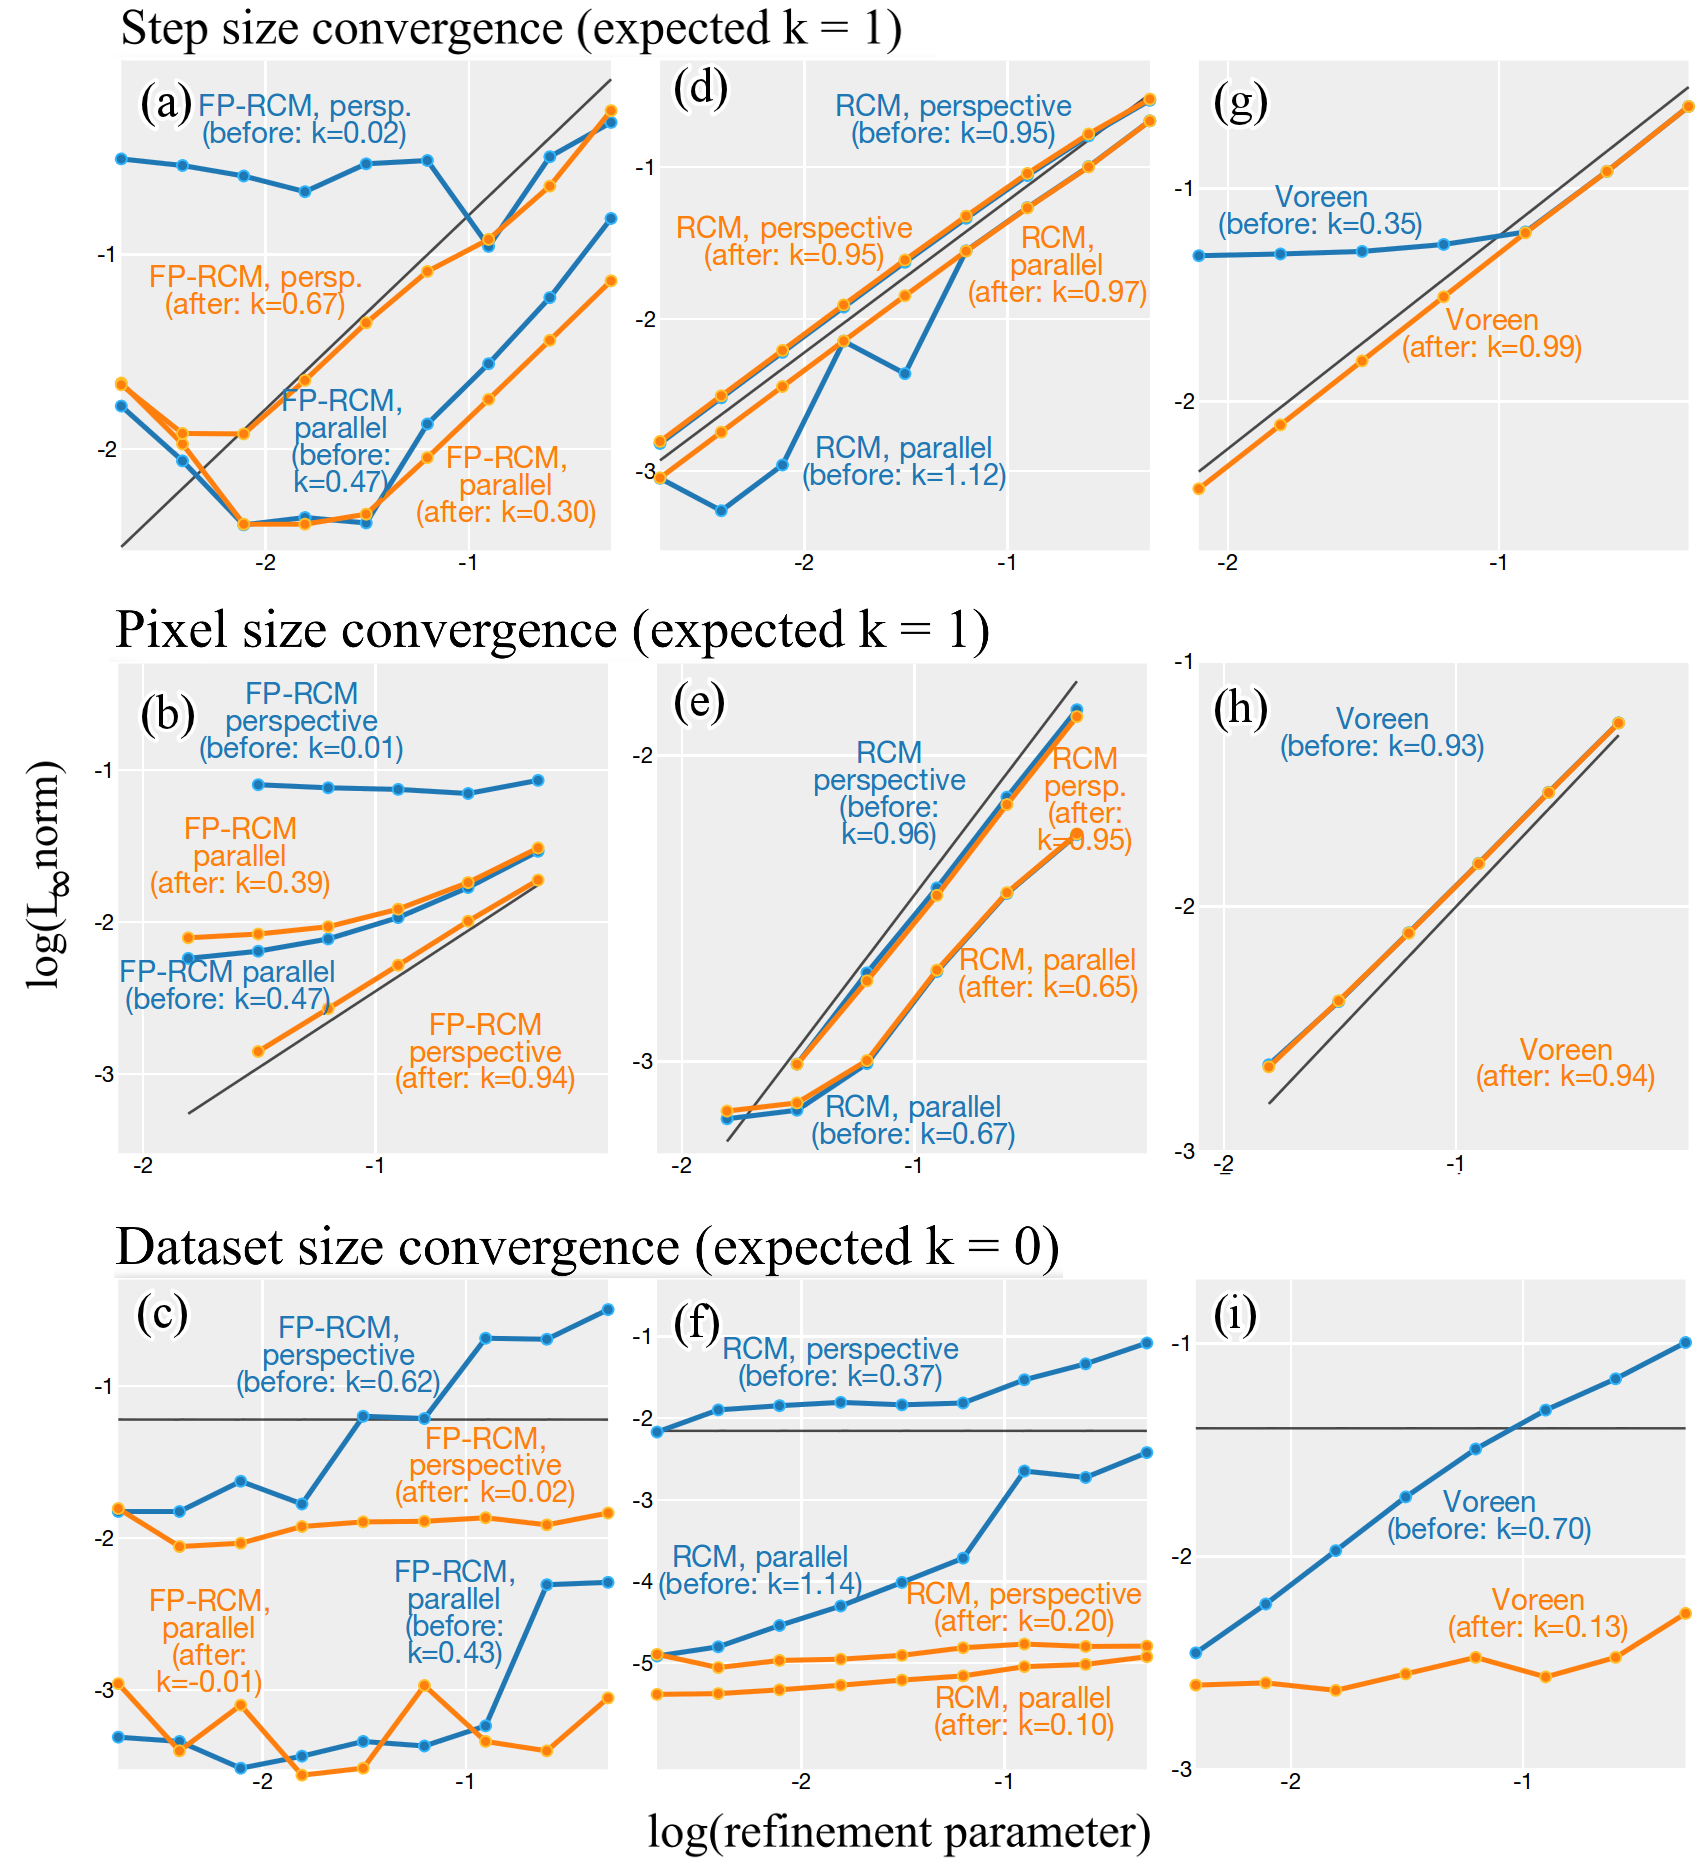
\includegraphics[width=0.85\linewidth]{chapter5/figures/convergence.png}
\caption{\label{fig:convergence} Each plot shows the convergence
  experiments for one particular implementation and one particular
  type of convergence. The behavior before any changes to the source
  code are shown in blue. The results of the changes are shown by the
  orange lines. The black line indicates the expected slope from the
  theoretical analysis. Notice the black lines indicate only the
  expected \emph{slope} of the results. Any line parallel to the black
  indicator line has the same slope and is equally acceptable.  The
  line slope value is denoted by $k$.
}
\end{figure}


\subsection{Observed behavior}

The results of our verification procedure are summarized in
Figure~\ref{fig:convergence}.  We tested both VTK and Voreen and found
unexpected behaviors.  We emphasize that this \emph{does not}
immediately translate into a code mistake but only that a deeper
analysis is needed. To find the reason for the unexpected behavior we
analyzed the source code of the given systems.  We expect linear
convergence when step size or pixel size are refined ($k = 1$) and
zeroth-order convergence when dataset refinement is used ($k = 0$).

\paragraph*{FP}
The results obtained for the FP module (blue curves in
Figures~\ref{fig:convergence}(a), (b), and (c)) were different from
expected for all tests. The 15-bit fixed-point precision could, to
some extent, justify this behavior. Still, we only expected this
influence to have a negative effect after a certain threshold for step
size. The perspective projection curve shown in
Figure~\ref{fig:convergence}(a), for instance, has zeroth-order
convergence when using step size refinement and perspective
projection. We expect convergence at least for large values of $d$
because when $d$ is too small, the errors due to 15-bit fixed-point
precision will dominate.
After investigating the reason for this deviation we found that
depending on the pixel position, some rays might cross only half of
the volume instead of the full volume. In other words, instead of
sampling the ray in $n$ locations, for some pixels the ray was only
sampled $\frac{n}{2}$ times. This is a combination of several factors
which includes domain size, step size, and ray direction. Details 
can be found in the supplementary material.

Using our synthetic dataset, we observed a `+' pattern shown in
Figure~\ref{fig:fp-rcm-example} (left). The darker regions are
precisely the pixels where the ray does not cover the whole
domain. Artifacts may also be seen in standard datasets such as the
Carp shown in Figure~\ref{fig:real-dataset-examples}.  The orange
curves in Figures~\ref{fig:convergence}(a), (b), and (c) show the
convergence results after modifying VTK's source.  Notice that for
step size refinement using perspective projection, the convergence
curve changed from $0.02$ to $0.92$ for the first seven samples. For the eigth 
and ninth samples the error slightly increases. A similar phenomenom occur
in the parallel convergence curve. The curve starts to
diverge in the high-resolution regime (parallel and perspective projection plot).
This might be due to the limit of 15-bit fixed point arithmetic.  Although 
the  pixel size refinement convergence for perspective projection substantially improved 
(from 0.01 to 0.94), the convergence curves for parallel projection remained similar. 
At this point, we do not know the source
of the discrepancy: the testing suite, the theory or the
implementation under verification.

\begin{figure}[t]
\centering
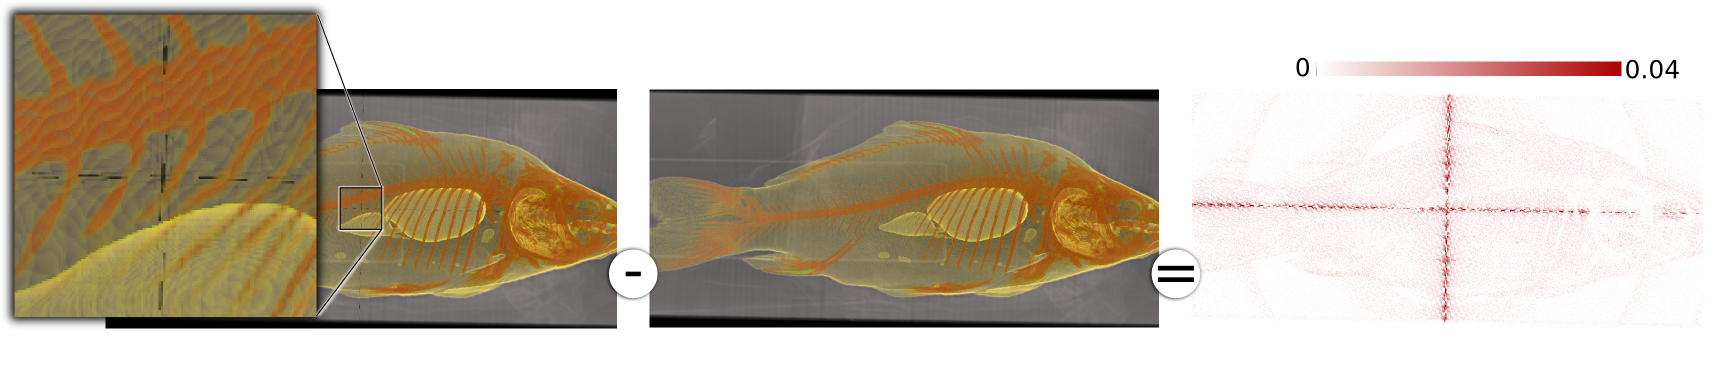
\includegraphics[width=1\linewidth]{chapter5/figures/carp-difference.png}
\caption{\label{fig:real-dataset-examples}
  A CT scan of a carp,
  rendered with VTK 5.6.1 and Fixed-Point Raycast Mapper (FP). On the
  left, we see the artifacts (dark lines) that prevented FP convergence. On the
  middle, we see the results after fixing the issues which prevented
  convergence. The artifacts are no longer visible. On the right we
  see the difference image.}
\end{figure}

\paragraph*{RCM}
The RCM module (blue curves in Figures \ref{fig:convergence}(d), (e),
and (f)) produces nearly linearly converging sequences when refining
the step size or pixel size.  However, dataset refinement with either
perspective or parallel projection fails to present the expected
zeroth-order convergence. Analyzing the source code, we found the
discrepancy to be due to the number of steps taken when marching
inside the volume. For instance, suppose that the step size is set in
such a way that 200 steps are required to traverse the volume. Instead
of 200 steps, the RCM module used from 195 to 199 steps, depending on
some conditions.  The consequence of this deviation 
is shown in Figure~\ref{fig:problem-example-01}.

The orange curves in Figures~\ref{fig:convergence}(d), (e), and (f)
show the convergence results for the RCM module after fixing the issue
that prevented code convergence. It consists of changing the epsilon
values used during the computation of the number of steps. Notice that
the behavior is close to the expected one and the errors are very
small ($10^{-5}$). The convergence curve using pixel size refinement
is close to linear for large pixel size but seems to be converging to
some positive value. This might be due to other sources of error which
become dominant after sufficient refinement.


\paragraph*{Voreen}

Our first ray refinement tests did not result in linear convergence
for Voreen (blue line in Figure~\ref{fig:convergence}(g)) due to the
early ray termination (ERT). By simply adapting the ERT threshold, we
were able to obtain the expected convergence for ray refinement
(orange line in the Figure~\ref{fig:convergence}(g)).

As can be seen in the Figure~\ref{fig:convergence}(i), the blue curve
indicates that increasing the resolution of the dataset decreases the
error.  We remind the reader that using our upsampled data, as
described in Section \ref{sec:VerViaDatasetRefinement}, rendering the
same scalar field represented by a different number of voxels should
not affect the result.  For Voreen, the unexpected behavior was caused
by sampling at incorrect texture locations.  More specifically,
internally, Voreen assumed that the texture data is node centered
when, in fact, OpenGL uses grid centered data. In this case, both the
volume and transfer function values were affected. In OpenGL, the
texture coordinates of a texture of resolution $R^m$ lie in the domain
$[0, 1]^m$, where $m$ is the texture dimension. Since the data values
are grid centered, this means that the outer most data values are
located at $[\frac{1}{2R}, 1-\frac{1}{2R}]$ with the settings used in
Voreen.  We will refer to the domain in which the data values lie, as
the data domain.  For volume rendering, the integration of a ray
should be done over the data domain, but for Voreen, the entry and
exit points of the rays went outside of that domain which caused the
unexpected behavior.  To obtain the expected constant convergence we
apply the following transformation to the input texture coordinate $p$
(see orange line in Figure~\ref{fig:convergence}(i)):

\begin{equation}
	p' = \frac{1}{2R} + p\left(1-\frac{1}{R}\right), p \in [0 \  1].
	\label{eq:correct_texture_sampling}
\end{equation}

Equation~\eqref{eq:correct_texture_sampling} scales and translates the
texture coordinate to be in the domain $[\frac{1}{2R},
  1-\frac{1}{2R}]^m$, where the data values lie.  The effect of
transforming the input coordinate for a real world example can be seen
in Figure~\ref{chap5:fig:teaser}.  We provide an explanation for why this
does not affect ray entry and exit point sampling, and also discuss
the implications of different boundary values in the supplementary
material.  Although the scaling of texture coordinates has been
addressed for multiresolution volumes~\cite{LjungLY06}, to our
knowledge, it has not been applied to the sampling of transfer
functions~\cite{Real-TimeVolumeGraphics06,Kruger03,Roettger03}.
%
There are other solutions for recovering the expected convergence
rate, which include changing the way we refine our sampling grid to
match OpenGL grid centered data.  However, we have chosen this
solution for several reasons. First, it matches Voreen's initial
assumption on node-centered data; it does not require special
treatment at the border of the domain; and due to its simplicity, it
is easy to implement.
%
We have contacted Voreen developers and the issue found was indeed
identified as a bug and the proposed solution will be adopted into
Voreen's next release.

No unexpected behavior could be detected for pixel size convergence as
shown in Figure~\ref{fig:convergence}(h), neither before nor
after changing the texture coordinate sampling. Both curves lie near 
the expected behavior (0.93 and 0.94).

\begin{figure}[b]
\centering
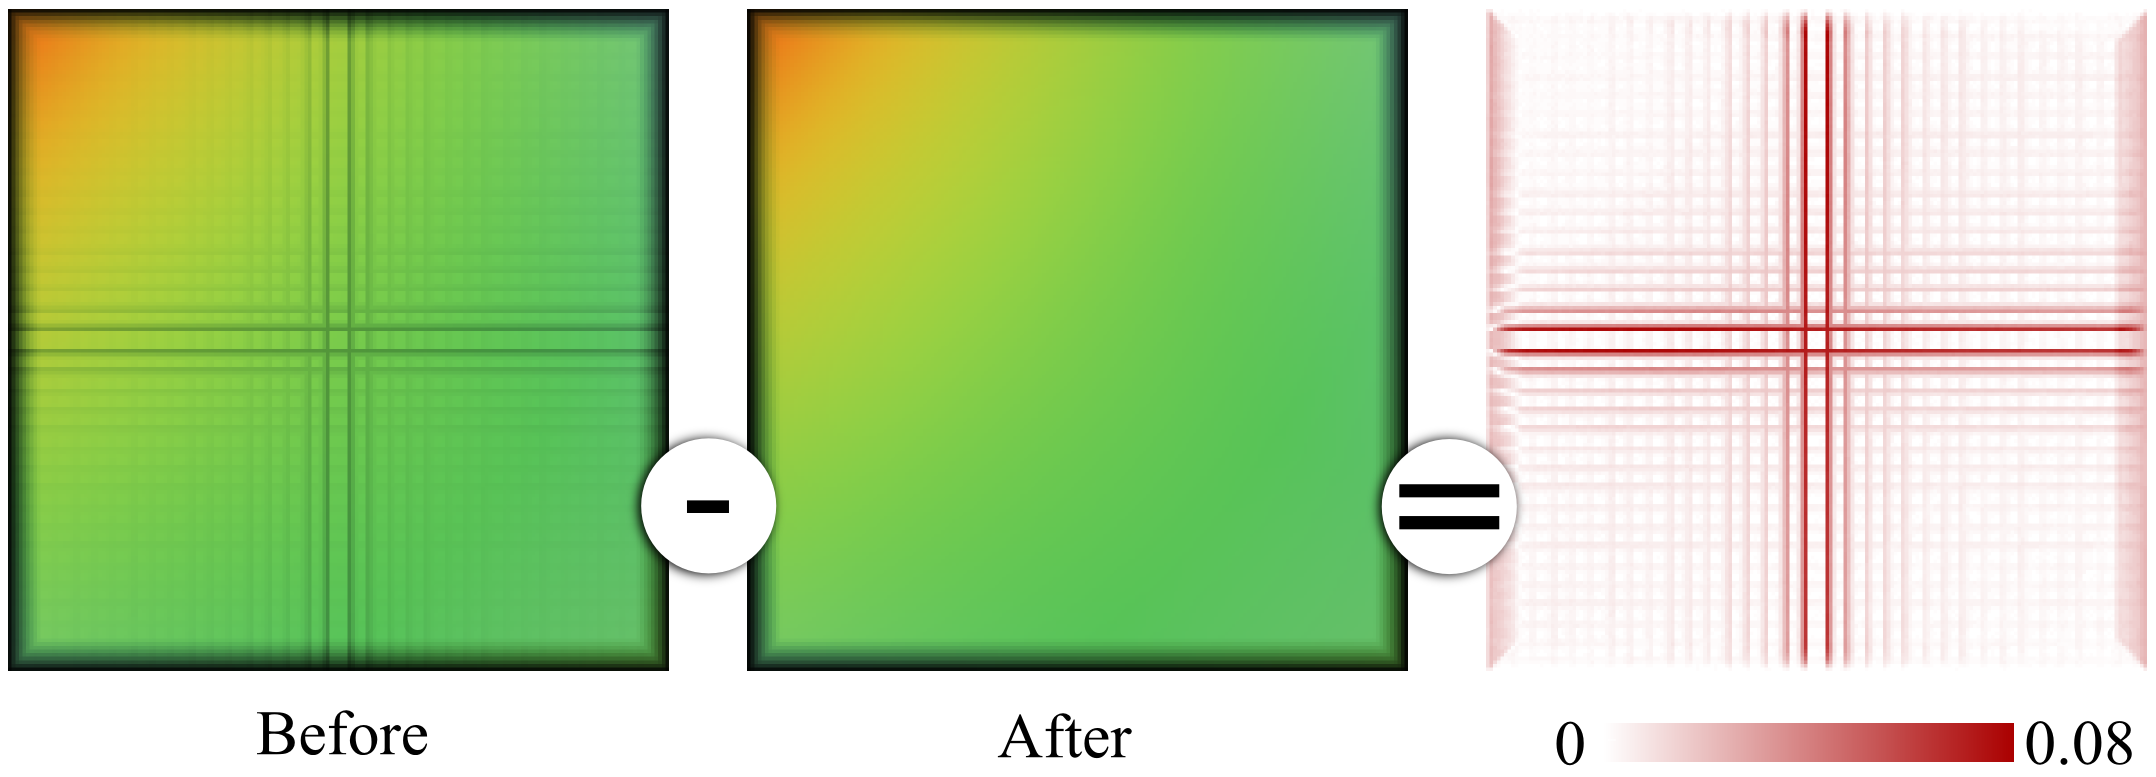
\includegraphics[width=0.98\linewidth]{chapter5/figures/fp-fcm-before-after.png}
\caption{\label{fig:fp-rcm-example} The figure shows images rendered
  using VTK 5.6.1. In our experiments, the `+'  pattern became more evident
  in two cases:  when coarse datasets are used; and/or high number
   of sampling points along the ray are used. 
   Darker pixels belong to regions where the
  ray traverses only half of the volume, preventing convergence. The
  image on the middle shows the result using our modified version of
  VTK. The convergence curve improved significantly. Note that this
  effect only occurs when perspective projection is used. For
  orthogonal projection, the problem is not noticeable. Step size
  convergence: Expected $k=1$. Before $k=1.2$.  After $k=1.2$.
  Dataset size convergence: Expected $k=0$. Before $k=-0.02$. After
  $k=-0.02$. Pixel size convergence: Expected $k=1$. Before $k=0.84$.
  After $k=0.85$. For the convergence analysis, we used a scalar field
  given by $S(x,y,z) = xyz$, $D=1$, transfer function $\tau(s) = s$ in the
  domain $\left[0,1\right]^3$, and solution for the VRI given by
  $I(x,y) = 1-\exp\left( -x y / 2 \right)$, which means the integration is 
  along $z$ (from zero to one).}
\end{figure}

\begin{figure}[b]
\centering 
\subfigure[Dataset refinement. Exp.: $k = 0$. Before:
  $k = 0.75$. After: $k = -0.18$]{
  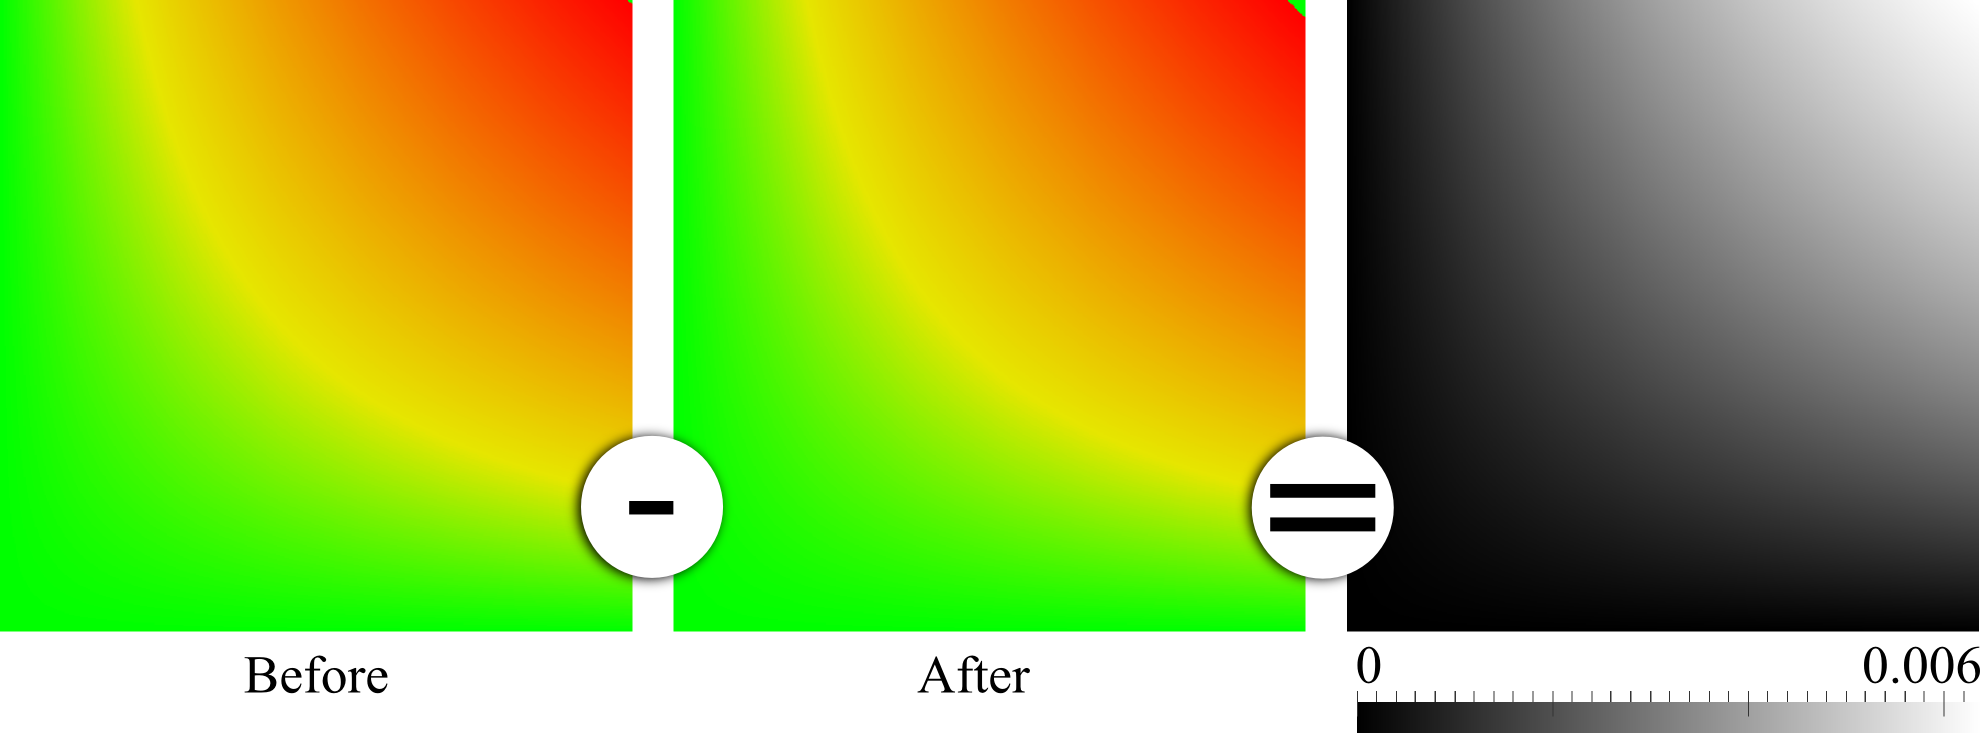
\includegraphics[width=0.98\linewidth]{chapter5/figures/problem-example-02.png}
  \label{fig:rcm-dataset}}
\subfigure[Pixel size refinement. Exp.: $k = 1$. Before:
  $k = 0.37$. After: $k = 1.23$]{
  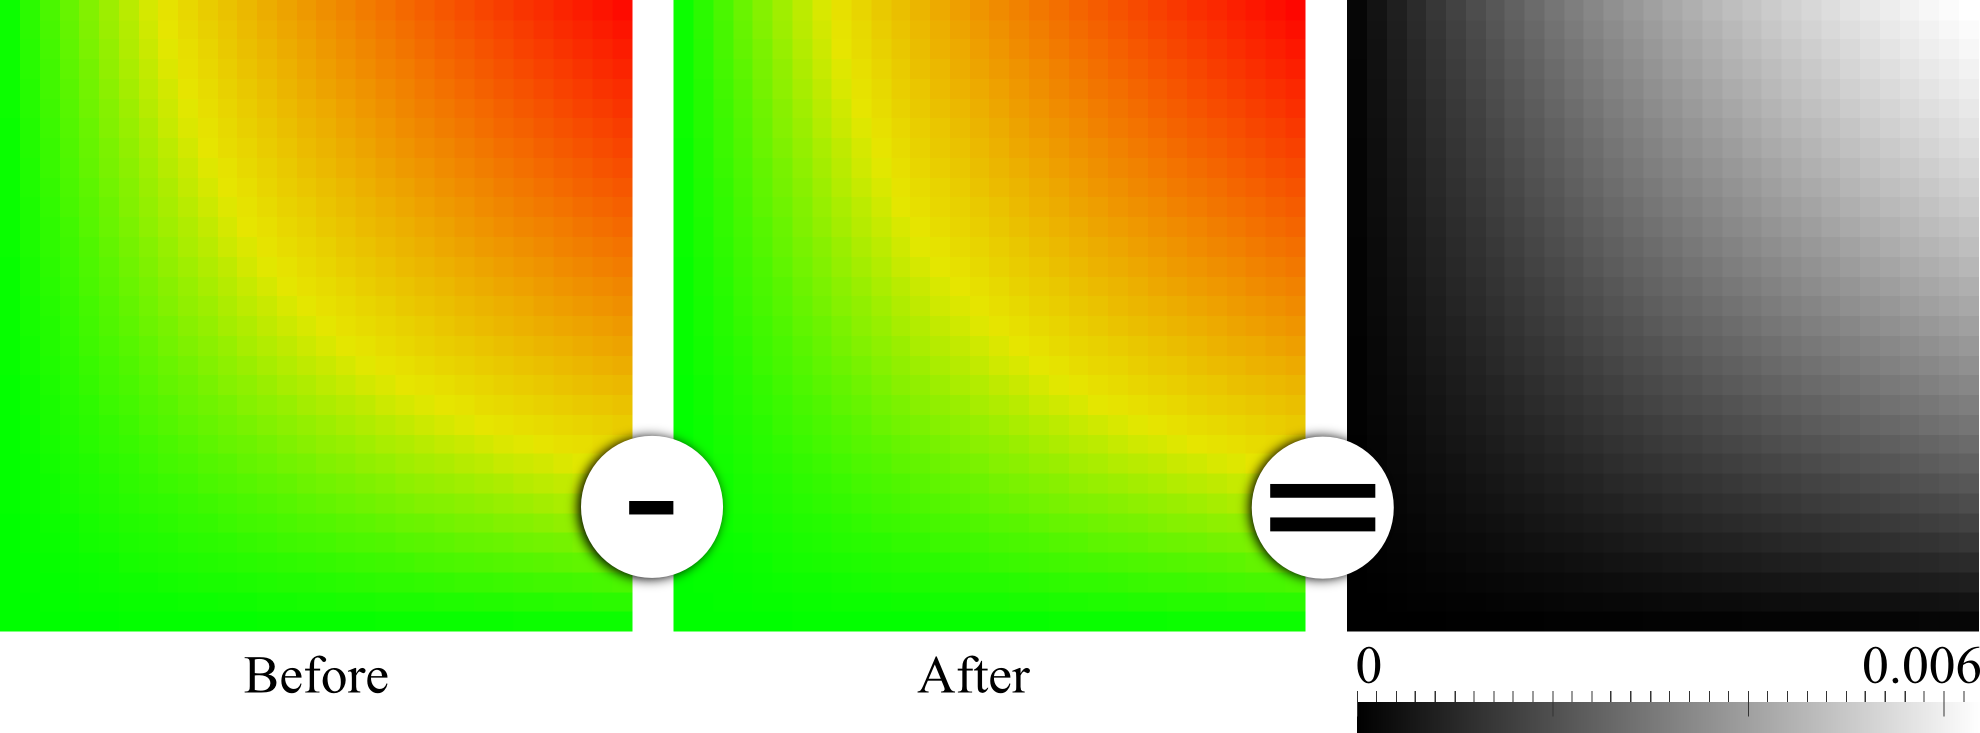
\includegraphics[width=0.98\linewidth]{chapter5/figures/problem-example-03.png}
  \label{fig:rcm-pixel}}
\caption{\label{fig:problem-example-01} The two figures show images
  rendered before and after fixing an issue with the number of ray
  samples in the RCM module. This change was motivated by a mismatch
  in the dataset convergence test. Although the images are
  indistinguishable to the human eye, the errors (computed as the
  difference between images, shown on the right) are large enough to
  change the expected convergence rate. For both images, we applied our
  verification procedures on a grid with a scalar field given by
  $S(x,y,z) = xyz$ and transfer function $\tau(s) = s$ in the domain
  $\left[0,1\right]^3$. Hence, the solution for the VRI is $I(x,y) =
  1-\exp\left( -x y / 2 \right)$. (a) uses dataset refinement while
  (b) uses pixel size refinement.}
\end{figure}


\section{Discussion}
\label{chap5:sec:discussion}

The convergence analysis presented in the previous section helped us
to identify unexpected behavior in two stable and widely used
frameworks. Unexpected behavior \emph{is not} indicative of an
implementation bug but rather a warning about potential problems. For
instance, some valid design decisions might affect the convergence
results. Consider the widely used ERT acceleration
technique. Depending on the thresholds involved, the convergence
results might deviate from the ideal, and the expected curve is
recovered once this feature is turned off. In this sense, the
verification tool can help the developer to identify portions of the
code that introduce numerical errors and quantify their effect on the
final image. The issue with the RCM module is another example. The
dataset size convergence curve was unexpectedly linear because of a
small variation in the number of steps. While this particular issue
might not be harmful, we were able to learn and reason about its
consequences \emph{after} the verification process was
done. Furthermore, ``minor'' bugs and even design decisions cannot be
ignored as they can mask more complex mistakes. Therefore, one will be
more confident after the design decisions that affect convergence are
``turned off'' and the expected convergence is recovered.  The FP
module, on the other hand, significantly deviates from the ideal
number of steps required to march inside the volume. Although we could
force VTK to march the expected number of steps, we are still
investigating possible solutions to and consequences of this issue.
To promote an unexpected behavior to a bug, we need interaction with
the developers of the code to confirm the code mistake, which was the
case with Voreen.  One should be aware of the discussed issues when
implementing a volume rendering algorithm as their consequences are
often not discussed in the
literature~\cite{Real-TimeVolumeGraphics06}.

\subsection{Test sensitivity}
\label{sec:test-sesitivity}

A verification technique ideally should be sensitive to any deviation
from the correct implementation. Unfortunately, in practice,
verification has limited scope, and we gain confidence if it helps us
understand the code behavior, test sensitivity, and reveal bugs. There
are several ways to attain this goal: Yang \emph{et al.} applied model
checking for filesystem verification and reported \emph{unknown}
bugs~\cite{Yang:2006:UMC:1189256.1189259};
Howden~\cite{Howden:1980:ASV:357103.357107} evaluated the efficacy of
dynamic and static testing for the detection of \emph{known} real bugs
of a mathematical library; Knupp and Salari \cite{KnuppSalari02}, on
the other hand, used the order-of-accuracy verification procedure to
uncover \emph{known} manufactured bugs in a proof-of-concept code.  In
software engineering, the process of evaluating a testing suite by
injecting defects into a program is known as \emph{mutation
  testing}~\cite{Riley:2009:BTL:1667105}.

We already presented the results of applying our verification
framework to two libraries and with our experiments we confirm the
previously reported sensitivity of convergence
analysis~\cite{Roy2005}. We went further to explore other scenarios in
volume rendering that may affect the convergence curve. Thus, in the
spirit of mutation testing, we created new versions of VTK which
contain known issues. Table \ref{tab:vs} shows the results of some of
the performed tests. In our experiments, we observed that some issues
did not affect the observed behavior.  The reason for this is that an
incomplete set of tests~\cite{KnuppSalari02} was performed, as shown
with test $\#10$ in Table \ref{tab:vs}. In that case a bug in the G
and B color lookup went unnoticed because our framework only used the
R channel. Once the verification framework includes all three
channels, the convergence drops to $0$, revealing an unexpected
behavior. For bug $\#9$, we swapped two of the polynomial coefficients
but they were equal for the scalar field used and thus it was not
detected. After changing the scalar field to $s(x,y,z) = 1xyz + 2xy +
3xz + \cdots$ the convergence curve no longer matches the expected one
and thus the bug is detected. Bug $\#11$ was introduced in a
matrix-vector multiplication routine which turned out to be dead
code. However, for bug $\#12$, the loop range was slightly incorrect
and it was not detected, even after additional changes to the
verification framework.

Aside from the defects injected into VTK, the following is a list of
details known to affect the convergence curve:
\emph{ERT}, as explained before;
\emph{opacity correction}, when using the analytical solution of the volume rendering integral;
\emph{hardcoded tolerance constants}, the famous ``epsilons'';
\emph{off-by-one} indexing problems (sometimes VTK does not render pixels in the first or last
column of an image);
\emph{improper volume sampling} (cell centered versus grid centered
scalar fields);
\emph{high-frequency transfer functions};
\emph{high-frequency scalar fields};
\emph{incorrect texture coordinate mapping}, as reported with Voreen;
\emph{inconsistent number of steps through the volume}, as reported
with FP and RCM; etc. % hey guys, etc. and \emph{\emph{et al.}.}. are never capitalized :)
From all the observed situations where the step/dataset/pixel size
convergence was affected, many of these are deliberate design
decisions, minor mistakes during the verification procedure or minor
problems with the implementation itself which can be easily fixed.
%
Note that those issues were not all inside the ray integration routine
itself, but in a variety of locations, spanning from pre-processing
steps to OpenGL texture sampling of data.
Our verification procedure was sensitive enough to detect all these
situations. 

We stress that our goal is to provide a methodology for verification
of volume rendering implementations. Specifically, our goal is neither
to compare different volume rendering implementations nor to entirely
explain the behavior of the examined implementations. The users of the
proposed framework are developers and practitioners who want or need
to identify potential problems.

\begin{landscape}
\begin{table}[b]
\caption{\label{tab:vs}This table shows the sensitivity of the convergence verification
for different scenarios in a volume renderer.
We applied our step size verification using
  a manufactured solution with a scalar field given by $S(x,y,z) = xyz +
  xy + xz + yz + x + y + z + 1$ and transfer function $\tau(s)$
  varying linearly from zero to one for $s \in [0, \max(S(x,y,z))]$. On
  the right, we show what part of the volume rendering algorithm was
  affected by the issue.  In the bottom, the first row shows the
  rendered images for each of the issues. The second row shows the
  error difference between the exact and rendered solutions. See
  Section \ref{sec:test-sesitivity} for an explanation of the
  undetected issues.}
\begin{minipage}[b]{0.45\linewidth}
\begin{tabular}{clc|c}
\hline
\multirow{2}{*}{\#} & \multirow{2}{*}{Issue} &
\multirow{2}{*}{Detected} & {Observed} \\
 & & & behavior ($k=$) \\
\hline
\bugnumber & Incorrect opacity accumulation                   & Yes & 0.0\\
\bugnumber & Incorrect ray increment                          & Yes & 0.0\\
\bugnumber & Small changes to early ray termination           & Yes & 0.1\\
\bugnumber & Piecewise constant $\tau$                        & Yes & 0.0\\
\bugnumber & Incorrect matrix-point multiplication            & Yes & 0.0\\
\bugnumber & Incorrect evaluation of trilinear interpolant    & Yes & 0.0\\
\bugnumber & Uninitialized pixel center offset                & Yes & 0.0\\
\bugnumber & Incorrect coefficients computation 1             & Yes & 0.0\\
\bugnumber & Incorrect coefficients computation 2             & No  & 1.0\\
\bugnumber & Incorrect color lookup                           & No  & 1.0\\
\bugnumber & Incorrect matrix-viewpoint multiplication        & No  & 1.0\\
\bugnumber & Incorrect loop range                             & No  & 0.95\\
%
\end{tabular}
\end{minipage}\hspace{0.5in}
\begin{minipage}[c]{0.45\linewidth}
\begin{codebox}
\Procname{$\proc{Volume Rendering}$}
\zi \For each pixel
\zi     \Do Find pixel center $(\#7)$
\zi         Transform rays to voxels space  $(\#5,\#11)$
\zi         \For each step along the ray $(\#12)$
\zi            \Do Compute interpolant coefficients $(\#8, \#9)$
\zi                Interpolate scalar values $(\#6)$
\zi                Retrieve color and opacity $(\#4,\#10)$
\zi                Compositing $(\#1)$
\zi                Increment sample position $(\#2)$
\zi                Check for early ray termination $(\#3)$
            \End
       \End
\end{codebox}
%
\end{minipage}
%
\begin{tabular}{ccccccccccccc}
\hline
 
\includegraphics[scale=0.4]{chapter5/figures/solution.png}                   &
 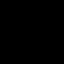
\includegraphics[scale=0.4]{chapter5/figures/wrong_opacity_accumulation.png} &
 
\includegraphics[scale=0.4]{chapter5/figures/wrong_ray_increment.png}        &
 
\includegraphics[scale=0.4]{chapter5/figures/early_ray_termination.png}      &
 
\includegraphics[scale=0.4]{chapter5/figures/piecewise_constant_alpha.png}   &
 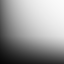
\includegraphics[scale=0.4]{chapter5/figures/wrong_matrix_point_multiplication.png}&
 
\includegraphics[scale=0.4]{chapter5/figures/incorrect_interpolant.png}&
 
\includegraphics[scale=0.4]{chapter5/figures/uninitialized_variable.png}&
 
\includegraphics[scale=0.4]{chapter5/figures/incorrect_coefficient_computation.png}&
 
\includegraphics[scale=0.4]{chapter5/figures/incorrect_coefficient_computation_2.png}&
 
\includegraphics[scale=0.4]{chapter5/figures/incorrect_color_lookup.png}     &
 
\includegraphics[scale=0.4]{chapter5/figures/wrong_matrix_viewpoint_mult.png}&
 
\includegraphics[scale=0.4]{chapter5/figures/wrong_loop_range.png}\\
\hline
 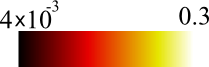
\includegraphics[scale=0.30]{chapter5/figures/legend-table.png} &
 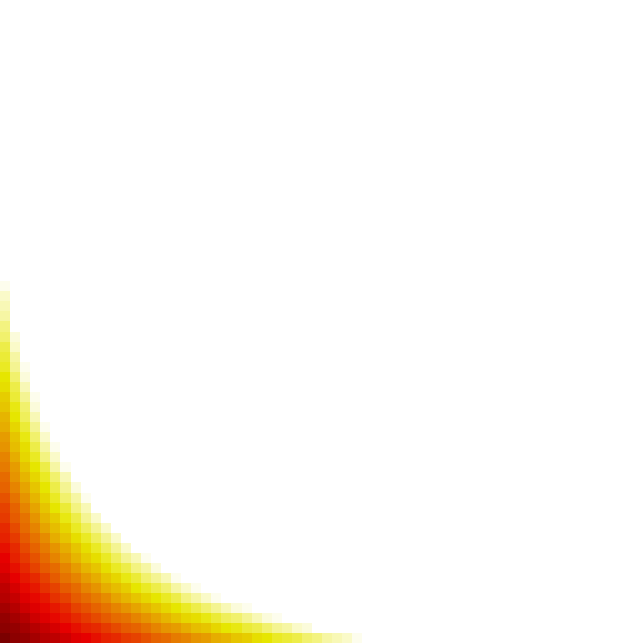
\includegraphics[scale=0.04]{chapter5/figures/wrong_opacity_accumulation-diff-2.png} &
 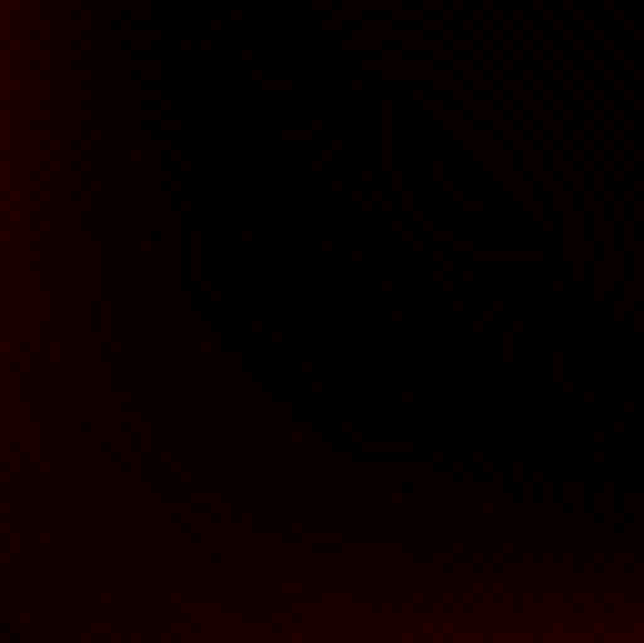
\includegraphics[scale=0.04]{chapter5/figures/wrong_ray_increment-diff-2.png}        &
 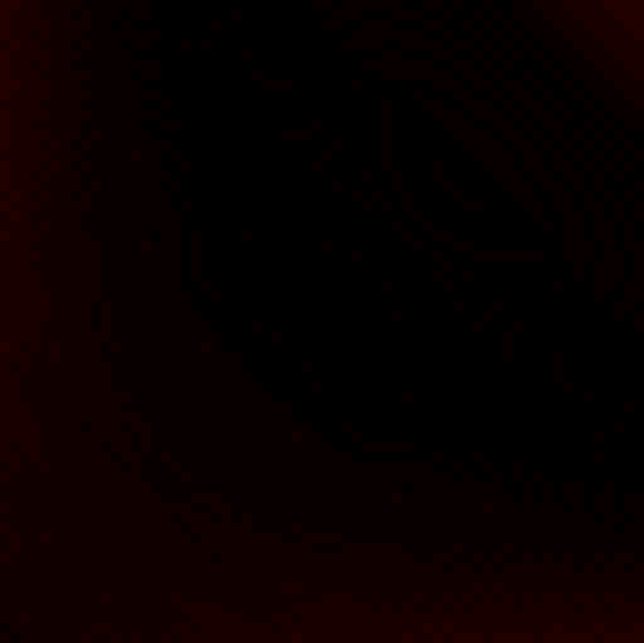
\includegraphics[scale=0.04]{chapter5/figures/early_ray_termination-diff-2.png}      &
 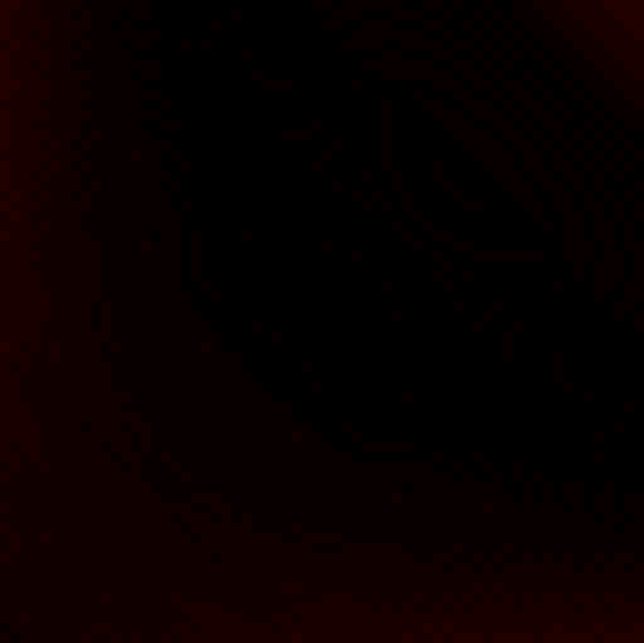
\includegraphics[scale=0.04]{chapter5/figures/piecewise_constant_alpha-diff-2.png}   &
 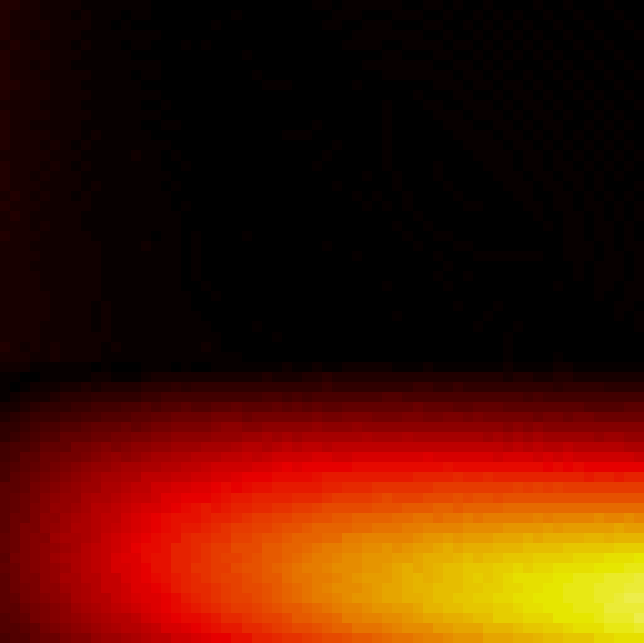
\includegraphics[scale=0.04]{chapter5/figures/wrong_matrix_point_multiplication-diff-2.png}&
 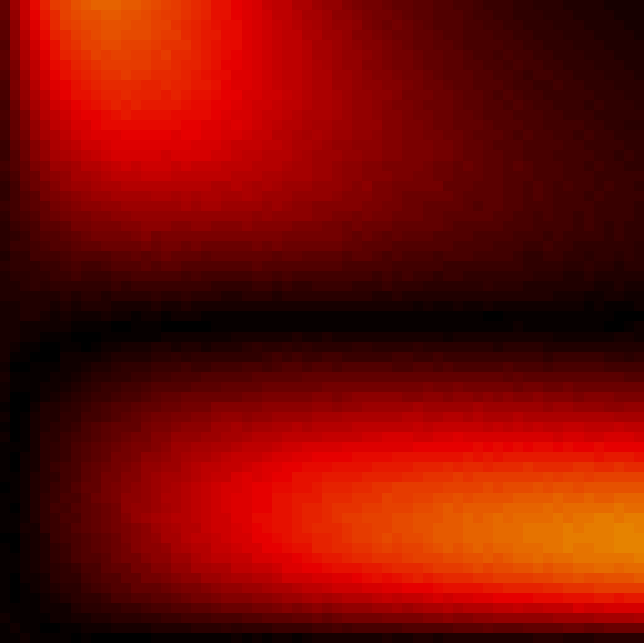
\includegraphics[scale=0.04]{chapter5/figures/incorrect_interpolant-diff-2.png}&
 
\includegraphics[scale=0.04]{chapter5/figures/uninitialized_variable-diff-2.png}&
 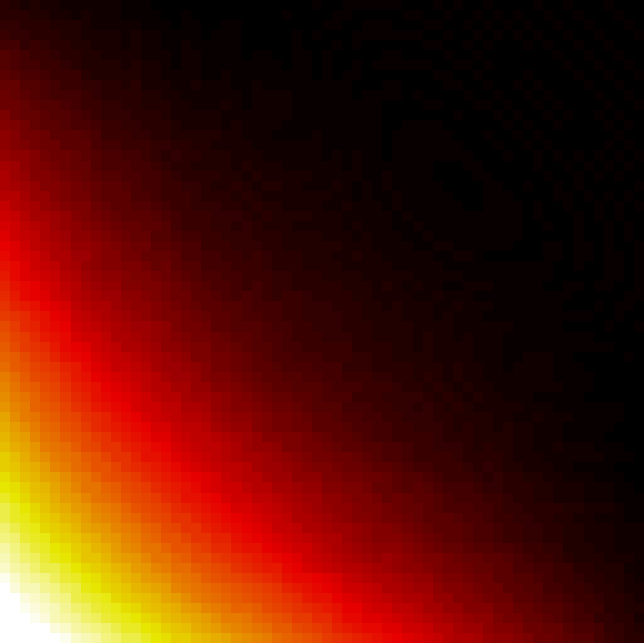
\includegraphics[scale=0.04]{chapter5/figures/incorrect_coefficient_computation-diff-2.png}&
 
\includegraphics[scale=0.04]{chapter5/figures/incorrect_coefficient_computation_2-diff-2.png}&
 
\includegraphics[scale=0.04]{chapter5/figures/incorrect_color_lookup-diff-2.png}     &
 
\includegraphics[scale=0.04]{chapter5/figures/wrong_matrix_viewpoint_mult-diff-2.png}&
 
\includegraphics[scale=0.04]{chapter5/figures/wrong_loop_range-diff-2.png}\\
\hline
Exact solution & 1 & 2 & 3 & 4 & 5 & 6 & 7 & 8 & 9 & 10 & 11 & 12\\
\end{tabular}
\end{table}
\end{landscape}

\subsection{Other volume rendering techniques}

While we focus on ray casting, our approach can be extended to other
techniques. Because the core of our method is a discretization of the
VRI, the only requirement is to formulate the volume rendering
algorithm as a numerical approximation to the true integral.
Splatting~\cite{Westover:1989:IVR:329129.329138}, for instance, uses a
reconstruction kernel before accumulating the contributions of voxels
into the final image. This approach is substantially different from
ray casting in the way it approximates the VRI, and so the asymptotic
errors involved will have to account for errors in both accumulation
and filter reconstruction~\cite{Moller:1996:CLE:236226.236235}.

Algorithmic improvements for volume rendering may require a more
careful approach. For example, pre-integration computes the results of
the integral with high precision over sample intervals and stores them
into a look-up table. This increases efficiency and quality, since
fewer steps are typically needed \cite{Engel01}. How the table
approximates the integral will affect the convergence rate: if there
is an analytical solution then no error is associated with $d$
intervals; otherwise, a numerical approximation scheme might be used
which means the error will depend on $d' = d / m$, where $m$ is the
number of sample points used in that interval and the integration
method used. For example, if a linear approximation is used for the
VRI during ray integration (instead of a standard sum of rectangles,
as done above), the final approximation should have second order
accuracy.

\subsection{Manufactured solutions}
%
In the interest of brevity, verification via pixel size and the
results presented in Table \ref{tab:vs} were generated from an
analytical solution for the volume rendering integral. Notice, still,
that the use of an analytical solution for verification is known as
the Method of Manufactured Solutions \cite{babuska04} and can be a
more rigorous procedure than convergence analysis alone
\cite{Roy2005}. In this way, we can verify that the results generated
by an implementation is converging with the right speed to the
\emph{correct solution}. The disadvantage lies in the difficulty of
designing manufactured solutions which are simultaneously simple (so
that we can write the theoretical convergence analysis down) and
sensitive (so that the experiment analysis catches bugs).

\section{Limitations}
\label{sec:limitations}
 
Both the discretization and verification procedures have
limitations. In the discretization of the VRI equation, we assume that
the solution $I(x,y)$ is smooth. Moreover, we assume that high-order
terms are negligible. This assumption implies that we can safely
discard all high-order terms when deriving the errors.  In addition,
the verification is done in a controlled fashion to avoid other error
sources, as shown in 
Figure \ref{fig:convergence}(a). Additional asymptotic analysis 
is necessary for each new error source. Also, $I$ must
be defined everywhere in the image plane. For instance, this condition
is violated if we change the camera position and orientation. One
needs to account for these transformation in $\mathbf{x}(\lambda)$, an
extra complication in the generation of analytical solutions.

The verification process has the same limitations previously described
but it also has practical limitations. For instance, one may be able
to observe that the convergence rate may not be the expected one for
low sampling rates. However, this is not due to the random scalar
field generated (which is a trilinear function and thus can be
represented exactly with the trilinear interpolant) but
high-frequency details in $\tau$ or $C$. This may lead to a violation
of the Nyquist rate. Because the process is iterative, for a correctly
implemented code, the expected convergence must be recovered once the
resolution is fine enough.  Another limitation is related to the number of
rays used per pixel. Many implementations can shoot several rays per
pixel, although this work assumes that only one ray is used. Also,
because the verification procedure considers the code as a blackbox,
it does not provide clues on the reasons for the unexpected behavior.

The scope of the mistakes that can be found by the verification
procedure is not clearly defined. All we can say is that it can find
bugs that actively affects the convergence of the
method~\cite{KnuppSalari02}. A common example of bugs that cannot be
found by this type of procedure is bugs that affect the
\emph{performance}: the code is slower due to the mistake but the
convergence is still the same~\cite{roach98}. The results shown in
Table \ref{tab:vs} is a first attempt to understand the scope of problems
that can be fixed by the verification procedure.

Currently, our verification procedure is focused on the solution for
the VRI without shading and other improvements on the final image
quality. Hence, if one wants to use our verification procedure in an
implementation that supports, for instance, shading, the feature will
need to be deactivated. Lastly, for the case of dataset refinement, we
assume that the underlying scalar field is defined by a piecewise-trilinear
function.

\section{Conclusion and Future Work}
\label{sec:conclusion}

In this chapter, we present verification techniques for volume rendering
based on the use of convergence analysis. Using these techniques, we
successfully found discrepancies in the behavior of the volume
rendering algorithms of two widely-used visualization packages.  We
note that we do not see our techniques as a replacement for the
currently used direct visual inspection or expert evaluations, but
instead as a way to complement those approaches, and lead to a more
comprehensive way to evaluate visualization software.  By providing
attractive quantitative alternatives, we hope to help make evaluation
of visualization software both easier and more effective, and also
contribute to a higher level of user trust in visual data analysis. We
believe the use of verification techniques will be of increasing
importance as the field of visualization matures and visualization
methods are used in a wide range of commercial and societal areas of
highest importance.

There is ample opportunity for future work. Extending our approach to
deal with volume shading and level-of-detail techniques would be
interesting and relevant research as these are widely used in
practice. Another important problem would be to explore the
verification of unstructured volume rendering techniques. Lastly,
there is room for improving the approximation error for
the three presented refinements. In addition, a new way for comparing
the convergence curves that allows one to gain insight on the
correctness of the implementation under verification is another
welcomed step.
